\documentclass{article}
\usepackage{l2hmc}
\usepackage{import}

\begin{document}

% TITLEPAGE {{{
\title{\textbf{Overview of the L2HMC Algorithm}\footnote{Source code can be
    found at: \url{https://github.com/saforem2/l2hmc-qcd}}}
\author{Sam Foreman\thanks{foremans@anl.gov, Argonne National Laboratory}\\
        James Osborn\thanks{osborn@alcf.anl.gov, Argonne National Laboratory}\\
      Xiao-Yong Jin\thanks{xjin@anl.gov, Argonne National Laboratory}}
\date{\today}
\maketitle
% }}}

\section{Introduction}%
\label{sec:l2hmc_intro}
We describe a new technique for performing Hamiltonian Monte-Carlo
(HMC) simulations called: `Learning to Hamiltonian Monte Carlo'
(L2HMC)~\cite{2017arXiv171109268L} which expands upon the traditional HMC by
using a generalized version of the leapfrog integrator that is parameterized by
weights in a neural network.
%
Hamiltonian Monte-Carlo improves upon the random-walk guess and check strategy
of generic MCMC by integrating Hamilton's equations along approximate
iso-probability contours of phase space.
%
In doing so, we are able to explore
the phase space more efficiently by taking larger steps between proposed
configurations while maintaining high acceptance rates.
%
In order to demonstrate the usefulness of this new approach, we use various
metrics for measuring the performance of the trained (L2HMC) sampler vs.\ the
generic HMC sampler.

First, we will look at applying this algorithm to a two-dimensional Gaussian
Mixture Model (GMM).
%
The GMM is a notoriously difficult distribution for HMC due to the vanishingly
small likelihood of the leapfrog integrator traversing the space between the
two modes.
%
Conversely, we see that through the use of a carefully chosen training
procedure, the trained L2HMC sampler is able to successfully discover the
existence of both modes, and mixes (`tunnels') between the two with ease. 
%
Additionally, we will observe that the trained L2HMC sampler mixes much faster
than the generic HMC sampler, as evidenced through their respective
autocorrelation spectra.

This ability to reduce autocorrelations is an important metric for measuring
the efficiency of a general MCMC algorithm, and is of great importance for
simulations in lattice gauge theory and lattice QCD.\@
%
Following this, we introduce the two-dimensional $U(1)$ lattice gauge theory
and describe important modifications to the algorithm that are of particular
relevance for lattice models.
%
Ongoing issues and potential areas for improvement are also discussed,
particularly within the context of high-performance computing and long-term
goals of the lattice QCD community.
%%%%%%%%%%%%%%%%%%%%%%%%%%%%%%%%%%%%%%%%%%%%%%%%%%%%%%%%%%%%%%%%%%%%%%%%%%%%%%%

\section{Hamiltonian Monte Carlo}%
\label{sec:l2hmc_hmc}
We can improve upon the random-walk guess and check strategy of the generic
Markov Chain Monte Carlo algorithm by ``guiding'' the simulation according to
the systems natural dynamics using a method known as Hamiltonian (Hybrid)
Monte Carlo (HMC).

In HMC, model samples can be obtained by simulating a physical system
governed by a Hamiltonian comprised of kinetic and potential energy functions
that govern a particles dynamics.
%
By transforming the density function to a potential energy function and
introducing the auxiliary momentum variable $v$, HMC lifts the target
distribution onto a joint probability distribution in phase space $(x, v)$,
where $x$ is the original variable of interest (e.g.\ position in Euclidean
space).
%
A new state is then obtained by solving the equations of motion for a fixed
period of time using a volume-preserving integrator (most commonly the
\emph{leapfrog integrator}).
%
The addition of random (typically normally distributed) momenta encourages
long-distance jumps in state space with a single Metropolis-Hastings (MH)
step.

Let the `position' of the physical state be denoted by a vector $x
\in\mathbb{R}^{n}$ and the conjugate momenta of the physical state be denoted
by a vector $v \in\mathbb{R}^{n}$.
%
Then the Hamiltonian reads
%
\begin{align}
  H(x, v) &= U(x) + K(v)\\
                    & = U(x) + \frac{1}{2} v^{T} \,v,
  \label{eq:hamiltonian}
\end{align}
%
where $U(x)$ is the potential energy, and $K(v)=\frac{1}{2}v^{T}v$ the
kinetic energy.%
%
We assume without loss of generality that the position and momentum variables
are independently distributed.
%
That is, we assume the target distribution of the system can be written as
$\pi(x, v) = \pi(x) \pi(v)$.
%
Further, instead of sampling $\pi(x)$ directly, HMC operates by sampling from the
canonical distribution $\pi(x, v) = \frac{1}{Z} \exp(-H(x, v)) = \pi(x)
\pi(v)$, for some partition function $Z$ that provides a normalization factor.
%
Additionally, we assume the momentum is distributed according to an
identity-covariance Gaussian given by $\pi(v) \propto \exp{(-\frac{1}{2} v^{T} \,
v)}$ For convenience, we will denote the combined state of the system by $\xi
\equiv (x, v)$.
%
From this augmented state $\xi$, HMC produces a proposed state $\xi^{\prime} =
(x^{\prime}, v^{\prime})$ by approximately integrating Hamiltonian dynamics
jointly on $x$ and $v$.
%
This integration is performed along approximate iso-probability contours of
$\pi(x, v) = \pi(x) \pi(v)$ due to the Hamiltonians energy conservation.
%
\subsection{Hamiltonian Dynamics}%
\label{subsec:mcmc_hamiltonian_dynamics}
One of the characteristic properties of Hamilton's equations is that they
conserve the value of the Hamiltonian.
%
Because of this, every Hamiltonian trajectory is confined to an energy
\emph{level set},
%
\begin{equation}
H^{(-1)}(E) = \{x, v | H(x, v) = E\}.
\end{equation}
%
Our state $\xi = (x, v)$ then proceeds to explore this level set by integrating
Hamilton's equations, which are shown as a system of differential equations in
Eq.~\ref{eq:hamiltons_equations}.
% along wich the state $\xi = (x, v)$
% The state $\xi$ is modified in such a way that $H(\xi)$ remains constant thorughout the simulation.
%
% The differential equations governing the motion through state space are given by
%
\begin{align}
  \dot x_i &= \frac{\partial H}{\partial v_i} = v_i\\
  \dot v_i &= -\frac{\partial H}{\partial x_i} = - \frac{\partial
      U}{\partial x_i}
\label{eq:hamiltons_equations}
\end{align}
%
It can be shown~\cite{Neal_2012} that the above transformation is
volume-preserving and reversible, two necessary factors to guarantee asymptotic
convergence of the simulation to the target distribution.
%
The dynamics are simulated using the leapfrog integrator, which for a single
time step consists of:
%
\begin{align}
  v^{\frac{1}{2}} &= v - \frac{\eps}{2} \partial_x U(x)\\
  x^{\prime} &= x + \eps v^{\frac{1}{2}}\\
  v^{\prime} &= v - \frac{\eps}{2} \partial_x U(x^{\prime}).
  \label{eq:generic_leapfrog}
\end{align}
%
We write the action of the leapfrog integrator in terms of an operator
$\mathbf{L}: \mathbf{L}\xi \equiv \mathbf{L}(x, v) \equiv (x^{\prime},
v^{\prime})$, and introduce a momentum flip operator $\mathbf{F}: \mathbf{F}(x,
v) \equiv (x, -v)$.
%
The Metropolis-Hastings acceptance probability for the HMC proposal is given
by:
%
\begin{equation}
  A(\mathbf{F}\mathbf{L} \xi | \xi) = \min\left(1,
      \frac{\pi(\mathbf{F}\mathbf{L}\xi)}{\pi(\xi)}\left|
      \frac{\partial\left[\mathbf{F}\mathbf{L}\xi\right]}
      {\partial\xi^{T}}\right|\right),
\label{eq:metropolis_hastings}
\end{equation}
%
Where $\left|\frac{\partial\left[\mathbf{F}\mathbf{L}\xi\right]}
{\partial\xi^{T}}\right|$ denotes the determinant of the Jacobian describing
the transformation, and is equal to $1$ for traditional HMC.\@
%
In order to utilize these Hamiltonian trajectories to construct an efficient
Markov transition, we need a mechanism for introducing momentum to a given
point in the target parameter space.

Fortunately, this can be done by exploiting the probabilistic structure of the
system~\cite{Betancourt_2017}.
%
To lift an initial point in parameter space into one on phase space, we simply
sample from the conditional distribution over the momentum,
%
\begin{equation}
v \sim \pi(x | v).
\end{equation}
%
Sampling the momentum directly from the conditional distribution ensures that
this lift will fall into the typical set in phase space.
%
We can then proceed to explore the joint typical set by integrating Hamilton's
equations as demonstrated above to obtain a new configuration $\xi \rightarrow
\xip$.
%
We can then return to the target parameter space by simply projecting away the
momentum,
%
\begin{equation}
(x, v) \rightarrow x
\end{equation}
%
These three steps when performed in series gives a complete Hamiltonian Markov
transition composed of random trajectories that rapidly explore the target
distribution, as desired.
%
An example of this process can be seen in Fig~\ref{fig:hmc_phase_space}.
%
\begin{figure}[htpb]
\includegraphics[width=\textwidth]{new_figures/hmc_phase_space11}
\caption{\emph{Visualizing HMC for a $1D$ Gaussian} (example
  from~\cite{Betancourt_2017}, figure adapted with permission
  from~\cite{joeyl2hmc}). Each Hamiltonian Markov transition lifts the
  initial state onto a \color{gray}{random level set of the Hamiltonian,
  }\color{black} $H^{(-1)}(E)$, which can then be explored with a
  \color{blue}{Hamiltonian trajectory }\color{black} before
  \color{red}{projecting back down }\color{black} to the \color{green}{target
  parameter space}\color{black}.}%
\label{fig:hmc_phase_space}
\end{figure}
%
\vspace{-10pt}
\subsubsection{Properties of Hamiltonian Dynamics}
%
There are three fundamental properties of Hamiltonian dynamics which are
crucial to its use in constructing Markov Chain Monte Carlo updates.
%
\begin{enumerate}
  \item \textbf{Reversibility:} Hamiltonian dynamics are \textit{reversible}
      --- the mapping from $\mathbf{L}: \xi(t) \rightarrow \xi^{\prime} =
      \xi(t + s)$ is one-to-one, and consequently has an inverse
      $\mathbf{L}^{-1}$, obtained by negating the time derivatives in
      Eq.~\ref{eq:hamiltons_equations}.
  \item \textbf{Conservation of the Hamiltonian:} Moreover, the dynamics
      \textit{keeps the Hamiltonian invariant}.
  \item \textbf{Volume preservation:} The final property of Hamiltonian
      dynamics is that it \textit{preserves volume} in $(x, v)$ phase space
      (i.e. Liouville's Theorem).
\end{enumerate}
%
All in all, HMC offers noticeable improvements compared to the `random-walk'
approach of generic MCMC, but tends to perform poorly on high-dimensional
distributions.
%
This becomes immediately apparent when it is used for simulations in lattice
gauge theory and lattice QCD, where large autocorrelations and slow `burn-in'
can become prohibitively expensive.
%
%%%%%%%%%%%%%%%%%%%%%%%%%%%%%%%%%%%%%%%%%%%%%%%%%%%%%%%%%%%%%%%%%%%%%%%%%%%%%%%

%\begin{document}
\section{Generalizing the Leapfrog Integrator}%
\label{sec:generalizing_lf}
As in the HMC algorithm, we start by augmenting the current state $x \in
\mathbb{R}^n$ with a continuous momentum variable $v \in \mathbb{R}^{n}$ drawn
from a standard normal distribution.
%
Additionally, we introduce a binary direction variable $d \in \{ -1, 1\}$,
drawn from a uniform distribution. 
%
The complete augmented state is then denoted by $\xi \equiv (x, v, d)$, with
probability density $p(\xi) = p(x) p(v) p(d)$.
%
To improve the overall performance of our model, for each step $t$ of the
leapfrog operator $\mathbf{L}_{\theta}$, we assign a fixed random binary mask
$m^{t} \in{\{0, 1\}}^n$ that will determine which variables are affected by
each sub-update.
%
The mask $m^t$ is drawn uniformly from the set of binary vectors satisfying
$\sum_{i=1}^{n} m_{i}^{t} = \lfloor \frac{n}{2}\rfloor$, i.e.\ half the entries
of $m^t$ are $0$ and half are $1$.
%
Additionally, we write $\bar m^{t} = \mathbbm{1} - m^{t}$ and $x_{m^t} = x
\odot m^{t}$, where $\odot$ denotes element-wise multiplication, and
$\mathbbm{1}$ the vector of $1$'s in each entry.
%

We begin with a subset of the augmented space, $\zeta_1 \equiv (x, \partial_{x}
U(x), t)$, independent of the momentum $v$.
%
We introduce three new functions of $\zeta_1$: $T_v$, $Q_v$, and $S_v$.
%
We can then perform a single time-step of our modified leapfrog integrator
$\mathbf{L}_{\theta}$.
%

First, we update the momentum $v$, which depends only on the subset $\zeta_1$.
%
This update is written
%
\begin{equation}
\label{eq:update_momentum_forward1}
  \vp = v\, \odot
      \hspace{-1mm}
      \underbrace{\exp\left(\frac{\varepsilon}{2}S_{v}(\zeta_1)\right)}_{\text{%
      \footnotesize{\textbf{Momentum scaling}\normalsize}
       }}%
      \hspace{-1mm}
       - \frac{\varepsilon}{2}\bigg[\partial_{x}U(x)\odot
      \hspace{-1mm}
      \underbrace{\exp(\varepsilon Q_{v}(\zeta_1))}_{\text{%
       \footnotesize{\textbf{Gradient scaling}\normalsize}
        }}
       + \underbrace{T_v(\zeta_1)}_{\text{%
       \footnotesize{\textbf{Translation}\normalsize}
       }}\bigg]
\end{equation}
and the corresponding Jacobian is given by:
$\exp{\left(\frac{\eps}{2}\mathbbm{1} \cdot S_{v}(\zeta_1)\right)}$.
%
Next, we update $x$ by first updating a subset of the coordinates of $x$
(determined according to the mask $m^t$), followed by the complementary subset
(determined from $\bar m^{t}$).
%
The first update affects only $x_{m^{t}}$ and produces $x^{\prime}$.
%
This update depends only on the subset $\zeta_2 \equiv (x_{\bar m^t}, v, t)$.
%
Following this, we perform the second update which only affects
$x_{\bar{m}^t}^{\prime}$ and depends only on $\zeta_3 \equiv (x_{m^t}^{\prime},
v, t)$, to produce $x^{\prime\prime}$:
%
\begin{align}
  x^{\prime} &= x_{\bar{m}^t} + m^{t}\odot\left[x \odot \exp{(\eps
      S_x(\zeta_2))} + \eps\left(v^{\prime}\odot%
    \exp{(\eps Q_x(\zeta_2))} + T_x(\zeta_2)\right)\right]\\
  x^{\prime\prime} &= x^{\prime}_{m^t} + \bar m^t \odot \left[x^{\prime} \odot
    \exp{(\eps S_x(\zeta_3))} +%
    \eps\left(v^{\prime} \odot \exp{(\eps Q_x(\zeta_3))} +
  T_x(\zeta_3)\right)\right].
\end{align}
%
with Jacobians: $\exp{(\eps m^{t} \cdot S_x(\zeta_2))}$, and
$\exp{(\eps\bar{m^t}\cdot S_x(\zeta_3))}$, respectively. 
%
Finally, we proceed to update $v$ again, using the subset $\zeta_4 \equiv
(x^{\prime\prime}, \partial_{x} U^{\prime\prime}, t)$: 
%
\begin{equation} 
  \vpp = \vp \odot \exp\left(\frac{\varepsilon}{2} S_v(\zeta_4)\right) -
    \frac{\varepsilon}{2}\left[\partial_{x} U
  \odot \exp(\varepsilon Q_v(\zeta_4)) + T_v(\zeta_4)\right].
    \label{eq:update_momentum_forward2}
\end{equation}
%
In order to build some intuition about each of these terms, we discuss below
some of the subtleties contained in this approach and how they are (carefully)
dealt with.

The first thing to notice about these equations is that if $S_{i} = Q_{i} =
T_{i} = 0$ ($i = x, v$), we recover the previous equations for the generic
leapfrog integrator (as we would expect since we are attempting to
\emph{generalize} HMC).
%
We can also see a similarity between the equations for updating $v$ and those
for updating $x$: each update is generalized by \emph{scaling} the previous
value ($v$ or $x$), and \emph{scaling and translating} the updating value
(either $\partial_{x}\,U(x)$ or $x$).
%
It can be shown~\cite{2017arXiv171109268L}, that the scaling applied to the
momentum in Eq~\ref{eq:update_momentum_forward1} can enable, among other
things, acceleration in low-density zones to facilitate mixing between modes,
and that the scaling term applied to the gradient may allow better conditioning
of the energy landscape (e.g., by learning a diagonal inertia tensor), or
partial ignoring of the energy gradient for rapidly oscillating energies.

Second, note that because the determinant of the Jacobian appears in the
Metropolis-Hastings (MH) acceptance probability, we require the Jacobian of
each update to be efficiently computable (i.e.\ independent of the variable
actually being updated).
%
For each of the momentum updates, the input is a subset $\zeta = (x,
\partial_{x}\,U(x), t)$ of the augmented space and the associated Jacobian is
$\exp{\left(\frac{\eps}{2}\mathbbm{1}\cdot S_{v}(\zeta)\right)}$ which is
independent of $v$ as desired.
%
For the position updates however, things are complicated by the fact that the
input $\zeta$ is $x$-dependent.
%
In order to ensure that the Jacobian of the $x$ update is efficiently
computable, it is necessary to break the update into two parts following the
approach outlined in \emph{Real-valued Non-Volume Preserving transformations
(RealNVP)}~\cite{dinhRealNVP}.
%
\subsection{Metropolis-Hastings Accept/Reject}
Written in terms of these transformations, the augmented leapfrog operator
$\mathbf{L}_{\theta}$ consists of $M$ sequential applications of the
single-step leapfrog operator $\mathbf{L}_{\theta} \xi = \mathbf{L}_{\theta}(x,
v, d) = (x^{\prime\prime\times M}, v^{\prime\prime\times M}, d)$, followed by
the previously-defined momentum flip operator $\mathbf{F}$ which flips the
direction variable $d$, i.e.\ $\mathbf{F}\xi = (x, v, -d)$.
%
Using these, we can express a complete molecular dynamics update step as
$\mathbf{FL}_{\theta}\xi = \xip$, where now the Metropolis-Hastings acceptance
probability for this proposal is given by
%
\begin{equation}
    A(\mathbf{F}\mathbf{L} \xi | \xi) = \min\left(1,
        \frac{p(\mathbf{F}\mathbf{L}\xi)}{p(\xi)}\left|
        \frac{\partial\left[\mathbf{F}\mathbf{L}\xi\right]}
            {\partial\xi^{T}}\right|\right),
\end{equation}
%
Where $\left|\frac{\partial\left[\mathbf{F}\mathbf{L}\xi\right]}
{\partial\xi^{T}}\right|$ denotes the determinant of the Jacobian describing
the transformation.

In contrast to generic HMC where
$\left|\frac{\partial\left[\mathbf{F}\mathbf{L}\xi\right]}
{\partial\xi^{T}}\right| = 1$, we now have non-symplectic transformations
(i.e.\ non-volume preserving) and so we must explicitly account for the
determinant of the Jacobian.
%
These non-volume preserving transformations have the effect of deforming the
energy landscape, which, depending on the nature of the transformation, may
allow for the exploration of regions of space which were previously
inaccessible.
%
\newcommand{\energyA}{\includegraphics[width=0.4\textwidth]{energy_landscape/original_energy_landscape.pdf}}
\newcommand{\energyB}{\includegraphics[width=0.4\textwidth]{energy_landscape/modified_energy_landscape.pdf}}
%
\begin{figure}
  \centering 
  \Huge
  \parbox{\widthof{\energyA}}{\energyA} $\overset{\mathcal{J}}{\longrightarrow}$
  \parbox{\widthof{\energyB}}{\energyB} 
  \normalsize
  \caption{Example of how the determinant of the Jacobian can deform the energy landscape.}
\end{figure}

To simplify our notation, introduce an additional operator $\mathbf{R}$ that
re-samples the momentum and direction, e.g.\ given $\xi = (x, v, d)$,
$\mathbf{R}\,\xi = (x, v^{\prime}, d^{\prime})$ where $v^{\prime} \sim
\mathcal{N}(0, I)$, $d^{\prime} \sim \mathcal{U}\left(\{-1, 1\}\right)$.
%
A complete sampling step of our algorithm then consists of the following two
steps:
%
\begin{enumerate}
    \item $\xi^{\prime} = \mathbf{FL}_{\theta} \,\xi$ with probability
        $A(\mathbf{FL}_{\theta}\,\xi|\xi)$ %(Eq.~\ref{eq:metropolis_hastings}),
        otherwise $\xi^{\prime} = \xi$.
    \item $\xi^{\prime} = \mathbf{R}\,\xi$.
\end{enumerate}
%
Note however, that for MH to be well-defined, this deterministic operator must
be \emph{invertible} and \emph{have a tractable Jacobian} (i.e.\ we can compute
its determinant).
%
In order to make this operator invertible, we augment the state space $(x, v)$
into $(x, v, d)$, where $d \in \{-1, 1\}$ is drawn with equal probability and
represent the direction of the update.
%
All of the previous expressions for the augmented leapfrog updates represent
the forward ($d = 1$) direction.
%
We can derive the expressions for the backward direction ($d = -1$) by
reversing the order of the updates (i.e.\ $\vpp \rightarrow \vp$, then $\xpp
\rightarrow \xp$, followed by $\xp \rightarrow x$ and finally $\vp \rightarrow
v$).
%
For completeness, we include in Sec.~\ref{sec:lf_forward} and
Sec~\ref{sec:lf_backward} all of the equations (both forward and backward
directions) relevant for updating the variables of interest in our augmented
leapfrog sampler.
\section{Forward Direction \texorpdfstring{$(d = 1)$}{(d = 1)}:}%
\label{sec:lf_forward}
% \vspace{-20pt}
\begin{align}
  \vp &= v \odot \exp{\left(\frac{\eps}{2}S_{v}(\zeta_{1})\right)}% 
        - \frac{\eps}{2}\left[\partial_{x}\,U(x)\odot \exp{\left(\eps
          Q_{v}(\zeta_{1})\right)}%
        + T_{v}(\zeta_{1})\right] \\
  \xp &= x_{\bar{m}^{t}} + m^{t}\odot \left[x \odot \exp{\left(\eps
    S_{x}(\zeta_{2})\right)}%
        + \eps\left(\vp\odot\exp{\left(\eps Q_{x}(\zeta_{2})\right)} 
          + T_{x}(\zeta_{2})\right)\right] \\
  \xpp &= x^{\prime}_{m^{t}} + \bar{m}^{t}\odot \left[\xp \odot \exp{\left(\eps
    S_{x}(\zeta_{3})\right)}%
        + \eps\left(\vp\odot\exp{\left(\eps Q_{x}(\zeta_{3})\right)} +
      T_{x}(\zeta_{3})\right)\right] \\
  \vpp &= \vp \odot \exp{\left(\frac{\eps}{2}S_{v}(\zeta_{4})\right)}%
        - \frac{\eps}{2}\left[\partial_{x}\,U(\xpp)\odot \exp{\left(\eps
          Q_{v}(\zeta_{4})\right)}%
          + T_{v}(\zeta_{4})\right]
\label{eq:forward_update}
\end{align} 
%
With $\zeta_{1} = (x, \partial_{x}\, U(x), t)$, $\zeta_{2} = (x_{\bar{m}^{t}},
v, t)$, $\zeta_{3} = (x^{\prime}_{m^{t}}, v, t)$, $\zeta_{4} = (\xpp,
\partial_{x}\, U(\xpp), t)$.
%%%%%%%%%%%%%%%%%%%%%%%%%%%%%%%%%%%%%%%%%%%%%%%%%%%%%%%%%%%%%%%%%%%%%%%%%%%%%%%
%
\section{Backward Direction \texorpdfstring{$(d = -1)$}{(d = -1)}:}%
\label{sec:lf_backward}
%
\begin{align}
  v^{\prime} &= {\left\{v + \frac{\eps}{2}\left[\partial_{x}\,U(x)\odot
        \exp{\left(\eps Q_{v}(\zeta_{1})\right)}%
    + T_{v}(\zeta_{1})\right]\right\}} \odot
    \exp{\left(-\frac{\eps}{2}S_{v}(\zeta_{1})\right)} \\
  \xp &= x_{m^{t}} + \bar{m}^{t}\odot%
    {\left[x - \eps{\left(\exp{\left(\eps Q_{x}(\zeta_{2})\right)}\odot \vp%
    + T_{x}(\zeta_{2})\right)}\right]}\odot \exp{\left(-\eps
    S_{x}(\zeta_{2})\right)} \\ 
  \xpp &= x_{\bar{m}^{t}} + m^{t}\odot%
    {\left[\xp - \eps{\left(\exp{\left(\eps Q_{x}(\zeta_{3})\right)}\odot \vp%
    + T_{x}(\zeta_{3})\right)}\right]}\odot \exp{\left(-\eps
    S_{x}(\zeta_{3})\right)} \\
  v^{\prime\prime} &= {\left\{\vp +
      \frac{\eps}{2}\left[\partial_{x}\,U(\xpp)\odot%
        \exp{\left(\eps Q_{v}(\zeta_{1})\right)}
  + T_{v}(\zeta_{1})\right]\right\}}\odot 
    \exp{\left(-\frac{\eps}{2}S_{v}(\zeta_{4})\right)}
\label{eq:backward_update}
\end{align}
%
With $\zeta_{1} = (x, \partial_{x}\, U(x), t)$, $\zeta_{2} = (x_{m^{t}}, v,
t)$, $\zeta_{3} = (x^{\prime}_{\bar{m}^{t}}, v, t)$, $\zeta_{4} = (\xpp,
\partial_{x}\, U(\xpp), t)$.
%%%%%%%%%%%%%%%%%%%%%%%%%%%%%%%%%%%%%%%%%%%%%%%%%%%%%%%%%%%%%%%%%%%%%%%%%%%%%%%
%
%%%%%%%%%%%%%%%%%%%%%%%%%%%%%%%%%%%%%%%%%%%%%%%%%%%%%%%%%%%%%%%%%%%%%%%%%%%%%%%
\section{Determinant of the Jacobian}
In terms of the auxiliary functions $S_{i}, Q_{i}, T_{i}$, we can compute the
Jacobian:
%
\begin{align}
  \log|\mathcal{J}| 
  &= \log\bigg|\frac{\partial{\left[\mathbf{FL}_{\theta}\xi\right]}}{\partial
  \xi^{T}}\bigg|\\
  &= d \sum_{t\leq N_{\mathrm{LF}}}
    {\left[\frac{\eps}{2} \mathbbm{1}\cdot S_{v}(\zeta_{1}^{t}) + \eps m^{t}
        \cdot S_{x}(\zeta_{2}^{t}) 
      + \eps \bar{m}^{t} \cdot S_{x}(\zeta_{3}^{t}) + \frac{\eps}{2}\mathbbm{1}
\cdot S_{v}(\zeta_{4}^{t})\right]}.  \end{align}
%
where $N_{\mathrm{LF}}$ is the number of leapfrog steps, and $\zeta_{i}^{t}$
denotes the intermediary variable $\zeta_{i}^{t}$ at time step $t$ and $d$ is
the direction of $\xi$, i.e.\ $d = 1 \,\, (-1)$ for the forward (backward)
update.
%%%%%%%%%%%%%%%%%%%%%%%%%%%%%%%%%%%%%%%%%%%%%%%%%%%%%%%%%%%%%%%%%%%%%%%%%%%%%%%
%
%%%%%%%%%%%%%%%%%%%%%%%%%%%%%%%%%%%%%%%%%%%%%%%%%%%%%%%%%%%%%%%%%%%%%%%%%%%%%%%
%\end{document}

\section{Network Architecture}%
\label{subsec:l2hmc_network}
As previously mentioned, each of the functions $Q$, $S$, and $T$, are
implemented using multi-layer perceptrons with shared weights.
%
It's important to note that we keep separate the network responsible for
paramterizing the functions used in the position updates (`$\Xnet$', i.e.\
$Q_x$, $S_x$, and $T_x$), and the network responsible for parameterizing the
momentum updates (`$\Vnet$', i.e.\ $Q_v$, $S_v$, and $T_v$).
%
% Since both networks are identical, we describe the architecture of $\Vnet$
% below, and include a flowchart for $\Xnet$ illustrative purposes in
% Fig~\ref{fig:x_net_flowchart}.
%
\begin{figure}[htpb]
  \centering
  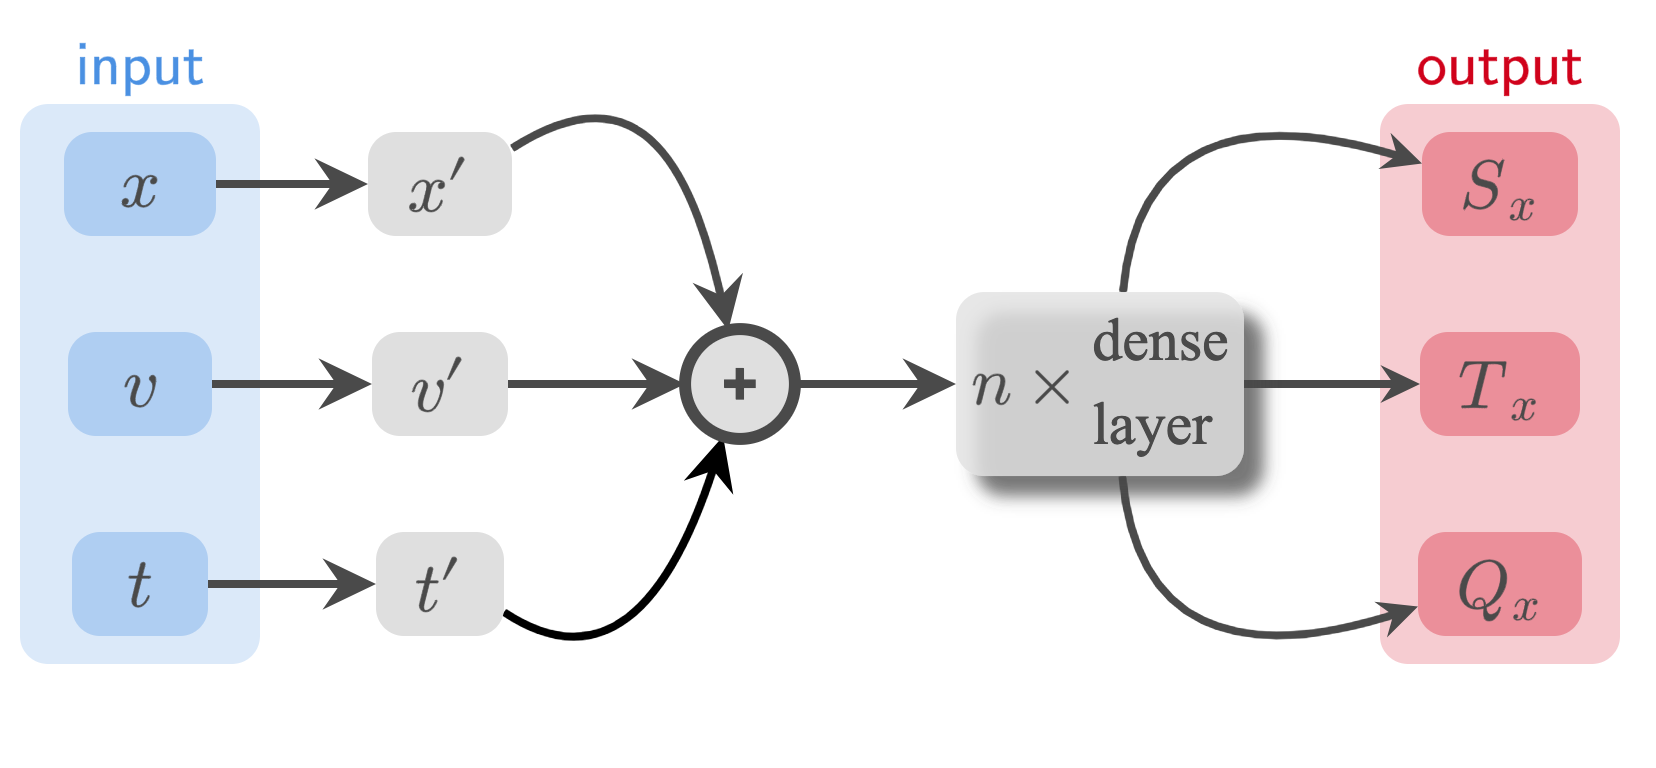
\includegraphics[width=\textwidth]{final/net.png}
  \caption{Illustration showing the generic (fully-connected) network
    architecture for training $S_x$, $Q_x$, and $T_x$.}%
    \label{fig:xnet}
\end{figure}

% \begin{figure}[htpb]
%   \centering
%   \input{tikz/vnet}
%   \caption{Illustration showing the generic (fully-connected) network
%     architecture for training $S_v$, $Q_v$, and $T_v$. Figure adapted
%     with permission from~\cite{joeyl2hmc}.}%
% \label{fig:generic_net}
% \end{figure}
%

The network takes as input $\zeta_1 = (x, \partial_{x} U(x), t)$, where $x, v
\in \mathbb{R}^{n}$, and $t$ is encoded as $\tau(t) = \left(\cos{(\frac{2\pi
t}{N_{\mathrm{LF}}})},\right.  \left.\sin{(\frac{2\pi
t}{N_{\mathrm{LF}}})}\right)$.
%
Each of the inputs is then passed through a fully-connected (`dense' layer),
consisting of $n_h$ hidden units
%
\begin{align}
    \tilde x &= W^{(x)} x + b^{(x)} \quad (\in \mathbb{R}^{n_h})\\
    \tilde v &= W^{(v)} v + b^{(v)} \quad (\in \mathbb{R}^{n_h})\\
    \tilde \tau &= W^{(\tau)} \tau + b^{(\tau)} \quad (\in \mathbb{R}^{n_h}).
\end{align}
%
Where $W^{(x)}, W^{(v)} \in \mathbb{R}^{n \times n_h}$, $W^{(t)} \in
\mathbb{R}^{2 \times n_h}$, and $b^{(x)}$, $b^{(v)}$,  $b^{(t)} \in
\mathbb{R}^{n_h}$.
%
From these, the network computes
%
\begin{equation}
    h_1 = \sigma(\tilde x + \tilde v + \tilde \tau) \quad (\in
    \mathbb{R}^{n_h}).
    \label{eq:hidden_1}
\end{equation}
%
Where $\sigma(x) = \max(0, x)$ denotes the rectified linear unit (ReLU)
activation function.
%
Next, the network computes
%
\begin{equation}
    h_2 = \sigma\left(W^{(h_1)} h_1 + b^{(h_1)}\right) \quad (\in
    \mathbb{R}^{n_h}).
    \label{eq:hidden_2}
\end{equation}
%
These weights ($h_2$) are then used to compute the network's output:
%
\begin{align}
    S_x &= \lambda_S \tanh(W^{(S)} h_2 + b^{(S)})\quad (\in \mathbb{R}^{n})\\
    Q_x &= \lambda_{Q} \tanh(W^{(Q)} h_2 + b^{(Q)})\quad (\in \mathbb{R}^{n})\\
    T_x &= W^{(T)} h_2 + b^{(T)}\quad (\in \mathbb{R}^{n}),
\end{align}
%
Where $W^{(s)}, W^{(q)}$, and $W^{(T)} \in \mathbb{R}^{n_h \times n}$ and
$b^{(s)}, b^{(q)}$, and $b^{(T)} \in \mathbb{R}^{n}$.
%
The parameters $\lambda_s$ and $\lambda_q$ are additional trainable variables
initialized to zero.
%
The network used for parameterizing the functions $T_v$, $Q_v$ and $S_v$ takes
as input $(x, \partial_x U(x), t)$ where again $t$ is encoded as above.  The
architecture of this network is the same, and produces outputs $T_v$, $Q_v$,
and $S_v$.

% \begin{figure}[htpb]
%   \centering
%   % \includegraphics[width=\textwidth]{generic_net/x_net_flowchart4.png}
%   % \input{tikz/vnet.tex}
%   \caption{Flowchart illustrating the generic fully-connected network
%     architecture including the intermediate variables computed at each hidden
%     layer of the network.}%
% \label{fig:x_net_flowchart}
% \end{figure}
%%%%%%%%%%%%%%%%%%%%%%%%%%%%%%%%%%%%%%%%%%%%%%%%%%%%%%%%%%%%%%%%%%%%%%%%%%%%%%%

%
%%%%%%%%%%%%%%%%%%%%%%%%%%%%%%%%%%%%%%%%%%%%%%%%%%%%%%%%%%%%%%%%%%%%%%%%%%%%%%%

\section{Training Procedure}%
\label{sec:training_procedure}

%
By augmenting traditional HMC methods with these trainable functions, we hope
to obtain a sampler that has the following key properties:
%
\begin{enumerate}
    \item Fast mixing (i.e.\ able to quickly produce uncorrelated samples).
    \item Fast burn-in (i.e.\ rapid convergence to the target distribution).
    \item Ability to mix across energy levels.
    \item Ability to mix between modes.
\end{enumerate}
%
Following the results in~\cite{10.2307/24308995}, we design a loss function
with the goal of maximizing the expected squared jumped distance (or
analogously, minimizing the lag-one autocorrelation).
%
To do this, we first introduce 
\begin{equation}
  \delta(\xi, \xip) = \delta((x^{\prime}, v^{\prime}, d^{\prime}), (x, v, d))
  \equiv \| x - x^{\prime}\|^2_2.  \label{eq:metric_orig}
\end{equation}
%
Then, the expected squared jumped distance is given by $\mathbb{E}_{\xi\sim
p(\xi)} \left[\delta(\mathbf{FL}_{\theta}\xi, \xi) A(\mathbf{FL}_{\theta}\xi |
\xi)\right]$.
%
By maximizing this objective function, we are encouraging transitions that
efficiently explore a local region of state-space, but may fail to explore
regions where very little mixing occurs.
%
To help combat this effect, we define a loss function
%
\begin{equation}
    \ell_{\lambda}(\xi, \xi^{\prime}, A(\xi^{\prime}|\xi)) =
        \frac{\lambda^2}{\delta(\xi,\xi^{\prime}) A(\xi^{\prime}|\xi)} -
        \frac{\delta(\xi,\xi^{\prime}) A(\xi^{\prime}|\xi)}{\lambda^2}
    \label{eq:loss_ell}
\end{equation}
%
where $\lambda$ is a scale parameter describing the characteristic length scale
of the problem.
%
Note that the first term helps to prevent the sampler from becoming stuck in a
state where it cannot move effectively, and the second term helps to maximize
the distance between subsequent moves in the Markov chain.  

The sampler is then trained by minimizing $\ell_{\lambda}$ over both the target
and initialization distributions.
%
Explicitly, for an initial distribution $\pi_0$ over $\mathcal{X}$, we define
the initialization distribution as $q(\xi) = \pi_0(x) \mathcal{N}(v; 0, I)
p(d)$, and minimize
%
\begin{equation}
    \mathcal{L}(\theta)\equiv \mathbb{E}_{p(\xi)}\left[\ell_{\lambda}(\xi,
    \mathbf{FL}_{\theta}\xi, A(\mathbf{FL}_{\theta}\xi|\xi))\right] + \lambda_b
    \mathbb{E}_{q(\xi)}\left[\ell_{\lambda}(\xi, \mathbf{FL}_{\theta}\xi,
    A(\mathbf{FL}_{\theta} \xi| \xi))\right].
    \label{eq:loss_L}
\end{equation}
%
For completeness, we include the full algorithm~\cite{2017arXiv171109268L} used
to train L2HMC in Alg.~\ref{alg:l2hmc}.
%
\begin{algorithm}[htbp]%
  % \centering
    \SetKwProg{Fn}{def}{\string:}{}%
    \SetKwFunction{Range}{range}%
    \SetKwFor{For}{for}{\string:}{}%
    \SetKwIF{If}{ElseIf}{Else}{if}{:}{elif}{else:}{}%
    \SetKwFor{While}{while}{:}{fintq}%
    \AlgoDontDisplayBlockMarkers\SetAlgoNoEnd%
    % \SetAlgoNoLine%
    \DontPrintSemicolon%
    \SetKwInOut{Input}{input}\SetKwInOut{Output}{output}%
    \caption{Training procedure for the L2HMC algorithm.}%
    \Input{%
      \vspace{-5pt}
      \begin{enumerate}
        \item A (potential) energy function, $U: \mathcal{X} \rightarrow
          \mathbb{R}$ and its gradient $\nabla_x U: \mathcal{X} \rightarrow
          \mathcal{X}$\
          \vspace{-10pt}
        \item Initial distribution over the augmented state space, $q$
          \vspace{-10pt}
        \item Number of iterations, $N_{\mathrm{train}}$
          \vspace{-10pt}
        \item Number of leapfrog steps, $N_{\mathrm{LF}}$
          \vspace{-10pt}
        \item Learning rate schedule, ${(\alpha_{t})}_{t\leq N_{\text{train}}}$
          \vspace{-10pt}
        \item Batch size, $N_{\mathrm{samples}}$
          \vspace{-10pt}
        \item Scale parameter, $\lambda$
          \vspace{-10pt}
        \item Regularization strength, $\lambda_b$
      \end{enumerate}
    }\;
    \vspace{-15pt}
    Initialize the parameters of the sampler, $\theta$\;
    Initialize ${\{\xi_{p^{(i)}}\}}_{i\leq N_{\mathrm{samples}}}$ from
    $q{(\xi)}$\; \For{$t = 0$ \KwTo\ $N_{\mathrm{train}}$}{%
      Sample a minibatch, ${\left\{\xi_{q}^{(i)}\right\}}_{i\leq
      N_{\mathrm{samples}}}$ from $q{(\xi)}$.\; $\mathcal{L}\leftarrow 0$\;
      \For{$i = 1$ \KwTo$N_{\mathrm{LF}}$} {%
          $\xi_{p}^{(i)} \leftarrow\ \mathbf{R}\,\xi_p^{(i)}$\;
          $\mathcal{L} \,\,\,\,\leftarrow\mathcal{L} +
          \ell_{\lambda}\left(\xi_p^{(i)}, \FLq\xi_p^{(i)}, A
            (\FLq\xi^{(i)}_p|\xi^{(i)}_p)\right) + \lambda_b
            \ell_{\lambda}\left(\xi^{(i)}_q, \FLq\xi^{(i)}_q,
            A (\FLq\xi^{(i)}_q|\xi^{(i)}_q)\right)$\;
          $\xi_p^{(i)} \leftarrow \FLq\xi^{(i)}_p$ with probability
        $A(\FLq\xi^{(i)}_p|\xi^{(i)}_p)$\; }%
      \vspace{2pt}
      $\theta\ \leftarrow\ \theta-\alpha_t \nabla_{\theta} \mathcal{L}$\;
    }%
\label{alg:l2hmc}
\end{algorithm}
%%%%%%%%%%%%%%%%%%%%%%%%%%%%%%%%%%%%%%%%%%%%%%%%%%%%%%%%%%%%%%%%%%%%%%%%%%%%%%%
    
%%%%%%%%%%%%%%%%%%%%%%%%%%%%%%%%%%%%%%%%%%%%%%%%%%%%%%%%%%%%%%%%%%%%%%%%%%%%%%%

\section{Gaussian Mixture Model}%
\label{sec:l2hmc_gmm}
%
The Gaussian Mixture Model (GMM) is a notoriously difficult example for
traditional HMC to sample accurately due to the existence of multiple modes.
%
In particular, HMC cannot mix between modes that are reasonably separated
without recourse to additional tricks.
%
This is due, in part, to the fact that HMC cannot easily traverse the
low-density zones which exist between modes.

In the most general case, we consider a target distribution described by a
mixture of $M > 1$ components in
$\mathbb{R}^{D}$ for $D \geq 1$:
%
\begin{equation}
    p(\mathbf{x}) \equiv \sum_{m=1}^{M} p(m) p(\mathbf{x}|m) \equiv
        \sum_{m=1}^{M} \pi_m p(\mathbf{x}|m) \quad \forall \,\,\mathbf{x} \in
        \mathbb{R}^{D}
    \label{eq:gmm_model}
\end{equation}
%
where $\sum_{m=1}^{M} \pi_m = 1$, $\pi_M \in (0, 1)$ $\forall m = 1, \ldots, M$
and each component distribution is a normal probability distribution in
$\mathbb{R}^{D}$.
%
So $\mathbf{x}|m \sim \mathcal{N}(\bm{\mu}_m, \bm{\Sigma}_m)$, where
$\bm{\mu}_m \equiv \mathbb{E}_{p{(\mathbf{x}|m)}}\left\{\mathbf{x}\right\}$ and
$\mathbf{\Sigma}_m \equiv \mathbb{E}_{p{(\mathbf{x}|m)}}{\left\{{(\mathbf{x} -
\bm{\mu}_m)}{(\mathbf{x} - \bm{\mu}_m)}^{T}\right\}} > 0$ are the mean vector
and covariance matrix, respectively, of component $m$.
%%%%%%%%%%%%%%%%%%%%%%%%%%%%%%%%%%%%%%%%%%%%%%%%%%%%%%%%%%%%%%%%%%%%%%%%%%%%%%%
%
%%%%%%%%%%%%%%%%%%%%%%%%%%%%%%%%%%%%%%%%%%%%%%%%%%%%%%%%%%%%%%%%%%%%%%%%%%%%%%%
\subsection{Example}
%
Consider a simple 2D case consisting of two Gaussians 
%
\begin{equation}
    \mathbf{x} \sim \pi_1 \,\mathcal{N}(\bm{\mu}_1, \bm{\Sigma}_1) +
        \pi_2\, \mathcal{N}(\bm{\mu}_2, \bm{\Sigma}_2)
    \label{eq:log_likelihood_example}
\end{equation}
%
with $\pi_1 = \pi_2 = 0.5$, $\bm{\mu}_1 = (-2, 0)$, $\bm{\mu}_2 = (2, 0)$ and
%
\begin{equation}
    \bm{\Sigma}_1 = \bm{\Sigma}_2 = 
        \begin{bmatrix}
            0.1    & 0 \\
            0       & 0.1 
        \end{bmatrix}
    \label{eq:covariance_matrix}
\end{equation}
%
The results of trajectories generated using both traditional HMC and the L2HMC
algorithm can be seen in Fig.~\ref{fig:gmm_trajectories}.
a
Note that traditional HMC performs poorly and is unable to mix between the two
modes, whereas L2HMC is able to correctly sample from the target distribution
without getting stuck in either of the individual modes.

%
The L2HMC sampler was trained using simulated annealing using the schedule
shown in Eq~\ref{eq:gmm_annealing} with a starting temperature of $T = 10$, for
$5,000$ training steps.
%
By starting with a high temperature, the chain is able to move between both
modes (`tunnel') successfully.
%
Once it has learned this, we can lower the temperature back to $T = 1$ and
recover the initial distribution while preserving information about tunneling
in the networks ``memory''.
%
\begin{equation}
  T(n) = {\left(T_{i} - T_{f}\right)} \cdot {\left(1 -
  \frac{n}{N_{\mathrm{train}}}\right)} + T_{f} 
\label{eq:gmm_annealing}
\end{equation}
%
\begin{figure}[htbp]
    \centering
    \includegraphics[width=\textwidth]{gmm_figures/iso_gmm_chains1}
    \caption{Comparison of trajectories generated using L2HMC (top), and
        traditional HMC with $\eps = 0.25$ (middle) and $\eps = 0.5$ (bottom).
        Note that L2HMC is able to successfully mix between modes, whereas HMC
        is not.}%
\label{fig:gmm_trajectories}
\end{figure}
%
\begin{figure}[htbp]
    \centering
    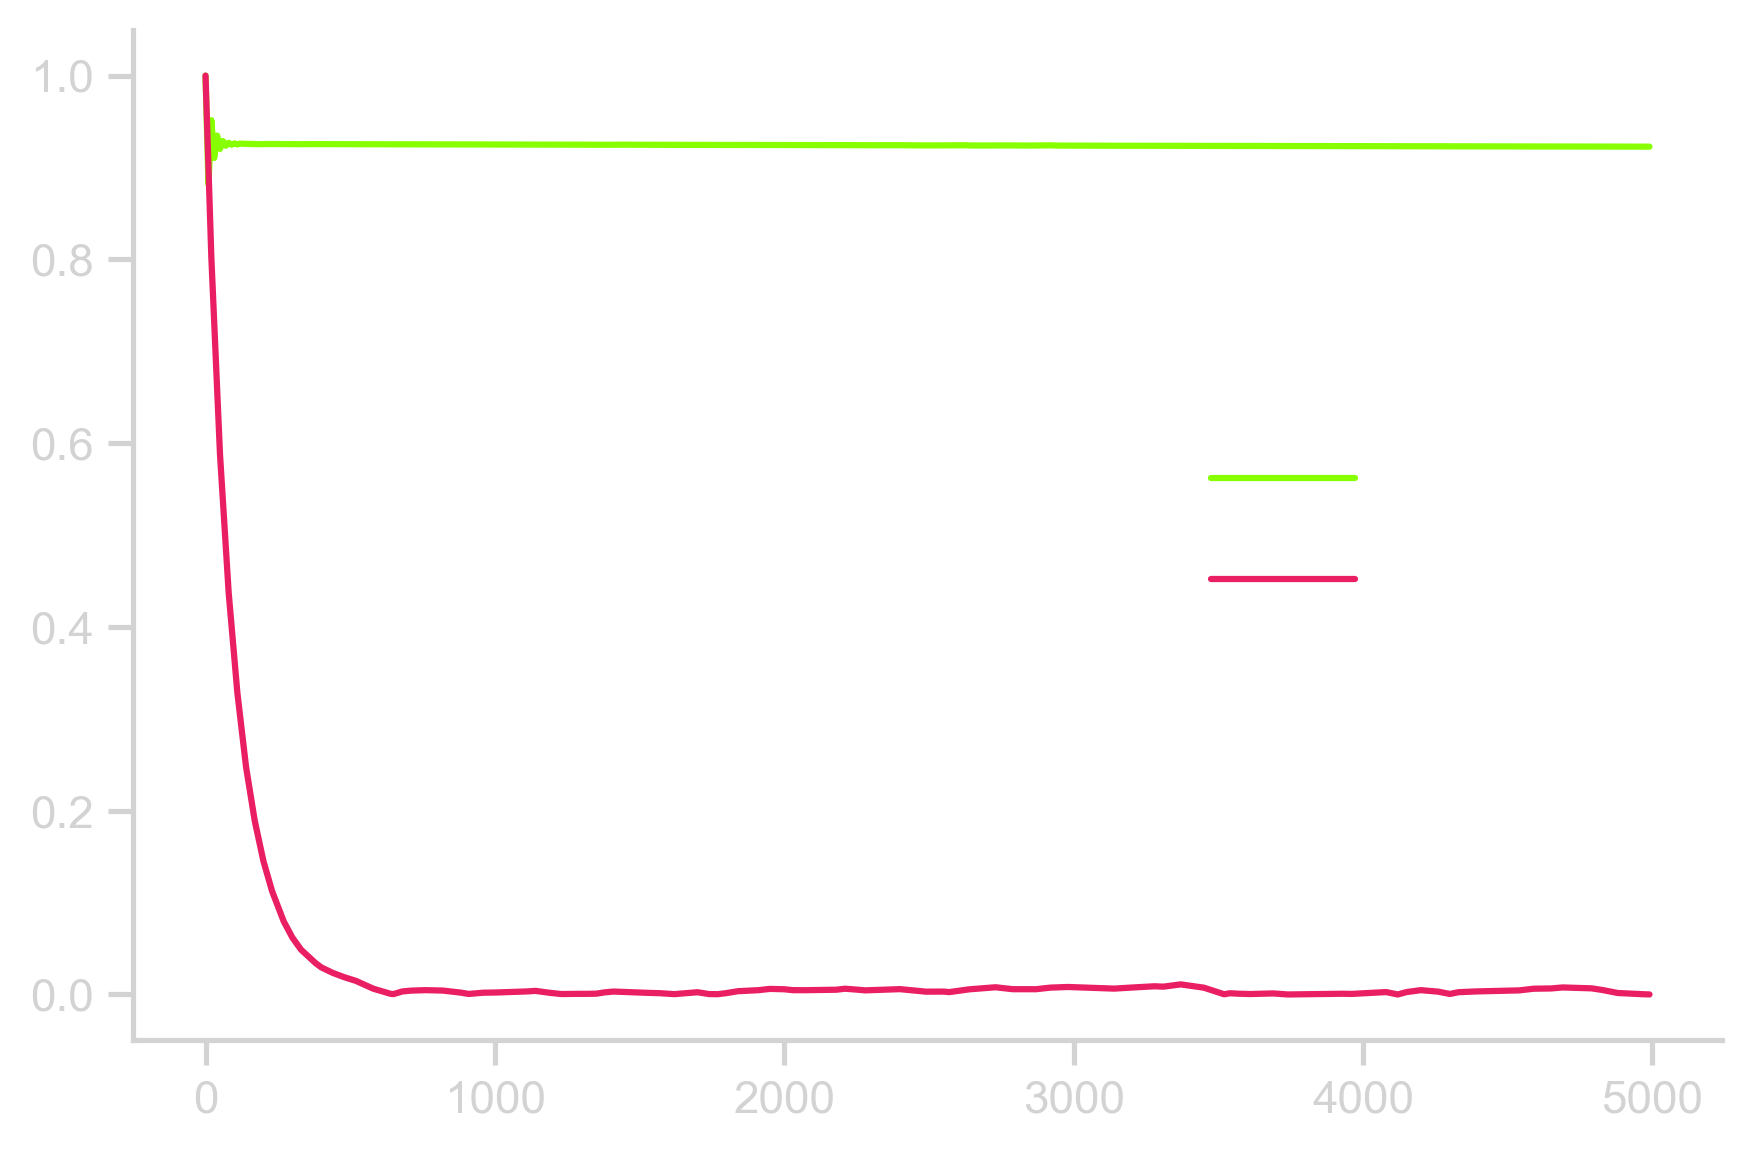
\includegraphics[width=0.98\textwidth]{gmm_figures/gmm_acl}
    \caption{Autocorrelation vs.\ gradient evaluations (i.e.\ MD steps). Note
    that L2HMC (blue) has a significantly reduced autocorrelation after the
  same number of gradient evaluations when compared to either of the two HMC
trajectories}% 
\label{fig:gmm_autocorrelation} 
\end{figure}
%%%%%%%%%%%%%%%%%%%%%%%%%%%%%%%%%%%%%%%%%%%%%%%%%%%%%%%%%%%%%%%%%%%%%%%%%%%%%%%
%

\section{2D \texorpdfstring{$U(1)$}{U (1)} Lattice Gauge Theory}%
\label{sec:l2hmc_u1} 
All lattice QCD simulations are performed at finite
lattice spacing $a$ and need an extrapolation to the continuum in order to be
used for computing values of physical quantities.
%
More reliable extrapolations can be done by simulating the theory at
increasingly smaller lattice spacings.
%
The picture that results when the lattice spacing is reduced and the physics
kept constant is that all finite physical quantities of negative mass dimension
diverge if measured in lattice units.
%
In statistical mechanics language, this states that the continuum limit is a
critical point of the theory since correlation lengths diverge.
%
MCMC algorithms are known to encounter difficulties when used for simulating
theories close to a critical point, an issue known as the \emph{critical slowing
down} of the algorithm.
%
This effect is most prominent in the topological charge, whose auto-correlation
time increases dramatically with finer lattice spacings.
%
As a result, there is a growing interest in developing new sampling techniques
for generating equilibrium configurations. 
%
In particular, algorithms that are able to offer improvements in efficiency
through a reduction of statistical autocorrelations are highly desired. 
%
We begin with the two-dimensional $U{(1)}$ lattice gauge theory with dynamical
variables $U_{\mu}{(i)}$ defined on the links of a lattice, where $i$ labels a
site and $\mu$ specifies the direction.
%
Each link $U_{\mu}{(i)}$ can be expressed in terms of an angle $0 <
\phi_{\mu}{(i)} \leq 2 \pi$.
%
\begin{equation}
    U_{\mu}{(i)} = e^{i\phi_{\mu}{(i)}}
    \label{eq:link_variable}
\end{equation}
%
with the Wilson action defined as:
%
\begin{equation}
    \beta S = \beta \sum_{P}{(1 - \cos{(\phi_{P})})}
    \label{eq:wilson_action}
\end{equation}
%
where
%
\begin{equation}
    \phi_{P} \equiv \phi_{\mu\nu}(i) = 
        \phi_{\mu}{(i)} + \phi_{\nu}{(i + \hat{\mu})} 
        - \phi_{\mu}{(i + \hat{\nu})} - \phi_{\nu}{(i)}
    \label{eq:phi_plaquette}
\end{equation}
%theta_
and $\beta = 1/e^{2}$ is the gauge coupling, and the sum $\sum_{P}$ runs over
all plaquettes of the lattice.
%
An illustration showing how these variables are defined for an elementary
plaquette is shown in Fig.~\ref{fig:plaquette}.
%
\begin{figure}[htpb]
  \centering
  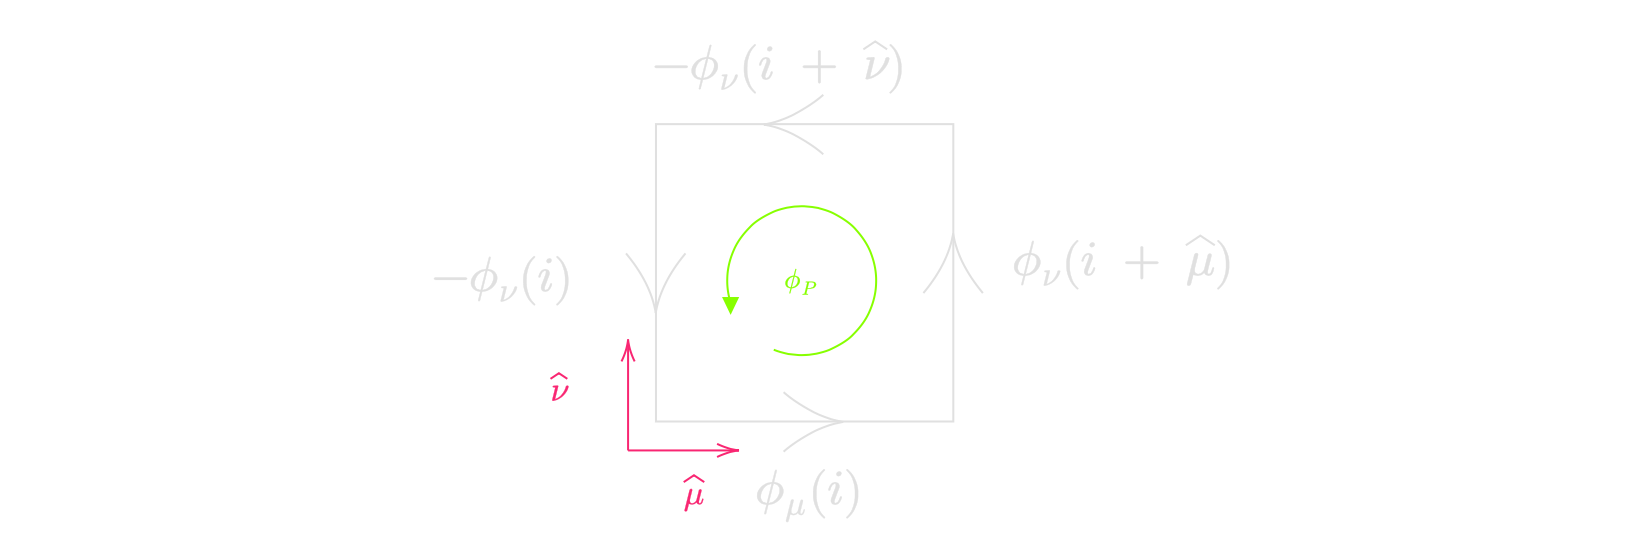
\includegraphics[width=0.5\textwidth]{gauge_figures/plaq.png}
  \caption{Illustration of an elementary plaquette on the lattice.}%
\label{fig:plaquette}
\end{figure}

We can define the topological charge, $\mathcal{Q} \in \mathbb{Z}$, as
%
\begin{equation}
  \mathcal{Q} \equiv \frac{1}{2\pi}\sum_{P} \tilde \phi_{P} =
    \frac{1}{2\pi}\sum_{\substack{{i; \mu, \nu}\\{\nu > \mu}}}
    \tilde \phi_{\mu\nu}{(i)}
    \label{eq:topological_charge}
\end{equation}
%
where
%
\begin{equation}
  \tilde{\phi}_{P} \equiv \phi_{P} - 2\pi {\bigg\lfloor{\frac{\phi_{P} +
  \pi}{2\pi}\bigg\rfloor}}
  % \tilde{\phi}_{P} \equiv \phi_{P} - 2 \pi \left \lfloor{\frac{\phi_{P} +
  % \pi}{2 \pi}\right \rfloor}
\end{equation}
%
is the sum of the link variables around the elementary plaquette, projected
onto the interval $\left[0, 2 \pi\right)$.
%
From this, we can define topological susceptibility
%
\begin{equation}
    \chi \equiv \frac{\langle \mathcal{Q}^2\rangle - \langle \mathcal{Q} \rangle^2}{V}
    % \label{eq:topological_susceptibility}
\end{equation}
%
By parity symmetry, $\langle \mathcal{Q} \rangle = 0$, so we have that
\begin{equation}
    \chi = \frac{\langle \mathcal{Q}^2\rangle}{V}
    \label{eq:topological_susceptibility}
\end{equation}
%
Unfortunately, the measurement of $\chi$ is often difficult due to the fact
that the autocorrelation time with respect to $\mathcal{Q}$ tends to be extremely long.
%
This is a consequence of the fact that the Markov chain tends to get stuck in a
topological sector (characterized by $\mathcal{Q} = const$.), a phenomenon known as
\emph{topological freezing}.
%
% (right) Topological charge vs.\ step generated using the trained
% L2HMC sampler.}%
\begin{figure}[htpb]
  \centering
    % \includegraphics[width=0.49\textwidth]{top_charge_vs_step_hmc.eps}
    % \includegraphics[width=0.49\textwidth]{top_charge_vs_step_l2hmc.eps}
    \includegraphics[width=0.6\textwidth]{charge_plots/top_charge_vs_step_HMC}
    % \includegraphics[width=0.49\textwidth]{charge_plots/compare/top_charge_vs_step_hmc}
    % \includegraphics[width=0.49\textwidth]{charge_plots/compare/top_charge_vs_step_l2hmc}
    \caption{Example of topological freezing in the $2D$ $U{(1)}$
      lattice gauge theory. The above result was generated using generic HMC
      sampling for a $8\times8$ lattice. Note that for the majority of the
      simulation $\mathcal{Q}=0$, making it virtually impossible to get a reasonable
    estimate of $\chi$.}\label{fig:top_charge} 
  \end{figure}
%
%
%%%%%%%%%%%%%%%%%%%%%%%%%%%%%%%%%%%%%%%%%%%%%%%%%%%%%%%%%%%%%%%%%%%%%%%%%%%%%%%
\subsection{Annealing Schedule}% 
\label{subsec:l2hmc_u1annealing}
% In addition to modifying the neural network architecture, we also modified
% the training algorithm to follow a simulated annealing schedule.
%
Proceeding as in the example of the Gaussian Mixture Model, we include a
simulated annealing schedule in which the value of the gauge coupling $\beta$
is continuously updated according to the annealing schedule shown in
Eq.~\ref{eq:annealing_schedule}.
%
% Explicitly, the value of the gauge coupling $\beta$ is continuously updated
% according to the annealing schedule shown in Eq.~\ref{eq:annealing_schedule}.
%
This was done in order to encourage sampling from multiple different
topological charge sectors, since our sampler is less `restricted' at lower
values of $\beta$.
%This was don
\begin{equation} 
  \frac{1}{\beta(n)} = {\left(\frac{1}{\beta_{i}} 
    - \frac{1}{\beta_{f}}\right)}
    {\left(\frac{1 - n}{N_{\mathrm{train}}}\right)} 
    + \frac{1}{\beta_{f}} 
\label{eq:annealing_schedule} 
\end{equation}
%
Here $\beta(n)$ denotes the value of $\beta$ to be used for the
$n^{\mathrm{th}}$ training step ($n = 1, \ldots, N_{\mathrm{train}}$),
$\beta_{i}$ represents the initial value of $\beta$ at the beginning of the
training, and $\beta_{f}$ represents the final value of $\beta$ at the end of
training.
%
For a typical training session, $N_{\mathrm{train}} = 25,000$, $\beta_{i} = 2$
and $\beta_{f} = 5$.
% For all of the exmaples above, $N_{\mathrm{train}} = 25,000$, $\beta_{0} = 2$
% and $\beta_{N_{\mathrm{train}}} = 5$.
%
% As can be seen in Fig.~\ref{fig:top_charge}

\subsection{Modified metric for \texorpdfstring{$U(1)$}{U (1)} Gauge
Model}%
\label{subsec:l2hmc_modifiedloss}
%
In order to more accurately define the ``distance'' between two different
lattice configurations, we redefine the metric in Eq.~\ref{eq:metric_orig} to
be
%
\begin{equation}
  % \delta(\xi(\phi_{\mu}(x)), \xip(\phi_{\mu}(x))) \equiv 1 -
  % \cos\left(\xi(\phi_{\mu}(x)) - \xi^{\prime}(\phi_{\mu}(x))\right)
  \delta(\xi, \xip) \equiv 1 - \cos\left(\xi - \xi^{\prime}\right)
\label{eq:new_metric}
\end{equation}
%
where now $\xi \equiv {\left(\phi_{\mu}^{x}(i), \,\phi_{\mu}^{v}(i),\,
d\right)}$, with $\phi_{\mu}^{x}$ representing the lattice of (`position')
gauge variables (what we called $x$ previously), and $\phi_{\mu}^{v}$
representing the lattice of (`momentum') gauge variables (what we called $v$
previously). Note that $i$ runs over all lattice sites\footnote{In what
  follows, we will refrain from explicitly including the site index and make
  the assumption that it implicitly extends over all sites on the lattice.} and
  $\mu=0, 1$ for the two dimensional case.
%
We see that this metric gives the expected behavior, since $\delta \rightarrow
0$ for $\xi \approx \xip$.

%%%%%%%%%%%%%%%%%%%%%%%%%%%%%%%%%%%%%%%%%%%%%%%%%%%%%%%%%%%%%%%%%%%%%%%%%%%%%%%
%
%%%%%%%%%%%%%%%%%%%%%%%%%%%%%%%%%%%%%%%%%%%%%%%%%%%%%%%%%%%%%%%%%%%%%%%%%%%%%%%
\subsection{Issues with the Average Plaquette}
%
When running inference using the trained sampler, an issue was encountered in
which the average plaquette, $\langle \phi_{P}\rangle$ seems to converge to a
value which is noticeably different from the expected value in the infinite
volume limit, and can be seen in Fig.~\ref{fig:bad_convergence}.
%
In order to quantify this unexpected behavior, we can calculate the difference
between the observed value of the average plaquette, $\langle \phi_{P}\rangle$
and the expected value $\phi_{P}^{(*)}$ (calculated from the infinite volume
limit):
% 
\begin{equation}
  {\delta_{\phi_P}}(\alpha_Q, N_{\mathrm{LF}}) \equiv \langle \phi_P\rangle -
  \phi_{P}^{(*)} \neq 0.
  % - \langle{\phi_{P}^{\mathrm{(exact)}}}\rangle \neq 0}.
\end{equation}
%
% Which allows us to quantify this difference.%


% Upon further testing, an issue was encountered in which the
% of the average plaquette
% $\langle \phi_{P}\rangle$ seems to converge to a value which is noticeably
% different from the expected value in the infinite volume limit.
%
% This behavior can be seen in Fig.~\ref{fig:bad_convergence}, and seems to
% depend on both the number of augmented leapfrog steps used by our integrator,
% as well as the `strength' of the topological loss term in
% Eq.~\ref{eq:topological_loss_term}.
%
% The parameters used in Fig~\ref{fig:bad_convergence} are as follows: $L = 8$,
% $N_{\mathrm{LF}} = 7$, and $N_{\mathrm{samples}} = 128$,
% and the sampler was trained for $N_{\mathrm{train}} = 1\times10^{4}$.
%
% In Fig~\ref{fig:good_convergence}, the only change was the weight factor for
% the topological charge term in the loss function $\alpha_{Q} = 0$.
%
\begin{figure}[htpb]%
  \centering
    \includegraphics[width=0.49\textwidth]{new_figures/plaq_error/plaqs_diffs_vs_step_l2hmc_lf16.pdf}
    \includegraphics[width=0.49\textwidth]{new_figures/plaq_error/plaqs_diffs_vs_step_hmc_lf16.pdf}
    % \includegraphics[width=0.49\textwidth]{plaq_plots/plaqs_diffs_vs_step_bad.pdf}
    \caption{Difference between the observed and expected value of the average
      plaquette, $\delta_{\phi_{P}}$, \textbf{(left)}: using the trained L2HMC
      sampler, and \textbf{(right)}: using generic HMC.}%
      % trained L2HMC sampler \textbf{(left)} and generic HMC \textbf{(right)} .
      % HMC result, obtained by setting $\alpha_{S} = \alpha_{Q} = \alpha{T} = 0$
      % \textbf{(right)}:
      % \ref{subsec:net_weights}).}%
\label{fig:bad_convergence}
\end{figure}%
%%%%%%%%%%%%%%%%%%%%%%%%%%%%%%%%%%%%%%%%%%%%%%%%%%%%%%%%%%%%%%%%%%%%%%%%%%%%%%%

\section{Debugging}%
\label{sec:debugging}%
\subsection{Net Weights}
\label{subsec:net_weights}
%
In an attempt to better understand the source of this unexpected behavior,
multiplicative weights (referred to as `nw' for `network weights' in
Fig.~\ref{fig:bad_convergence}) were introduced to scale the individual
contribution from each of the `learned' functions $S$, $T$, and $Q$,
explicitly:
%
\begin{align}
  S &\rightarrow \alpha_{S}\, S \\
  T &\rightarrow \alpha_{T}\, T \\
  Q &\rightarrow \alpha_{Q}\, Q.
\end{align}
%
By varying each of these weights individually allows us to selectively `tune'
how much each of these functions contribute when running inference on the
trained model.
%
Note that in the limit $\alpha_{S}, \alpha_{T}, \alpha_{Q} \rightarrow 0$, we
recover generic HMC, and as can be seen in Fig.~\ref{fig:bad_convergence},
the error in the average plaquette $\delta_{\phi_{P}} \simeq 0$, as expected.
%
As an additional sanity check, we looked at how the error in the average
plaquette behaves for different values of the weights $\alpha_{i}$ ($i = S, T,
Q$).
%
Explicitly, beginning with $\vec{\alpha} \equiv [\alpha_{S}, \alpha_{Q},
\alpha_{T}] = [0, 0, 0]$, we increase each of the weights one by one and compute
the average value of the plaquette difference.
%
For example, the blue line (Transformation $(Q)$ function) in
Fig.~\ref{fig:plaq_diff_vs_net_weights} was obtained by keeping both
$\alpha_{S}$ and $\alpha_{T}$ fixed and $0$ and varying $\alpha_{Q} \in
[0.1, 0.25, 0.5, 0.75, 1.0, 1.5, 2.0, 5.0]$, and similarly for $\alpha_{S}$ and
$\alpha_{Q}$.
%
\begin{figure}
  \centering
  \begin{subfigure}[t]{0.48\textwidth}
    \caption{$N_{LF} = 10$}
    \includegraphics[width=\textwidth]{new_figures/plaq_error/plaq_diff_vs_net_weights_lf10.pdf}
  \end{subfigure}
  % \vspace{2pt}
  % \hfill
  % \centering
  \begin{subfigure}[t]{0.48\textwidth}
    \caption{$N_{LF} = 12$}
    \includegraphics[width=\textwidth]{new_figures/plaq_error/plaq_diff_vs_net_weights_lf12.pdf}
  \end{subfigure}
  % \vspace{2pt}
  \begin{subfigure}[b]{0.48\textwidth}
    \caption{$N_{LF} = 16$}
    \includegraphics[width=\textwidth]{new_figures/plaq_error/plaq_diff_vs_net_weights_lf16.pdf}
  \end{subfigure}
  \caption{Plaquette difference $\delta_{\phi_{P}}$ for different values of the
    net weights $\vec{\alpha} \equiv [\alpha_{S}, \alpha_{T}, \alpha_{Q}]$.
    Note that $\delta_{\phi_{P}} \rightarrow 0$ as $\vec{\alpha} \rightarrow
  [0, 0, 0]$, as expected.}%
\label{fig:plaq_diff_vs_net_weights}
\end{figure}
%
These results seem to indicate that each of the individual functions contribute
separately to the error, with the scaling ($S$) and translation ($T$) functions
having the largest effect.
%  }}}
\subsection{Updates (11/11/2019)}
\begin{todolist}
  \item[\done] Ensure reproducibility across training/inference runs when
    using same input parameters.
    \begin{itemize}
      \item Essential for debugging the bias in the average plaquette.
      \item Somewhat tricky problem due to the fact that tensorflow 
        has two distinct methods of specifying a seed: graph-level and
        operation-level. Additionally, when using horovod for distributed
        training across multiple ranks, we must ensure that each rank gets a
        different seed otherwise they will all be training identical copies of
        the model.
    \end{itemize}

  \item[\done] Implement reversibility checker that ensures that the L2HMC
    dynamics (i.e.\ the augmented HMC sampler) is reversible.
    \begin{itemize}
      \item Starting with $\xi = (x, v, d)$, run the dynamics in the forward
        direction to get $\xi^{\prime}$. If $\mathbf{L}_{\theta}
        \xi =  \xi^{\prime}$, and $\mathbf{F} \xi = \mathbf{F} (x, v, d) = (x,
        v, -d)$, then a complete (invertible) update step can be written as
        $\mathbf{FL}_{\theta}\xi = \xi^{\prime}$.
        %
      \item If our sampler is reversible, running the dynamics backwards on
        $\xi^{\prime}$ should return us to the original state $\xi$. 
        %
        \begin{equation}
          \mathbf{FL}_{\theta}\mathbf{FL}_{\theta} \xi = \xi
        \end{equation}
    \end{itemize}

  \item[\done] Try increasing floating point precision (\texttt{tf.float32 -->
    tf.float64}) (\textbf{\textcolor{red}{Error still present.}}) 

  \item[\done] Try anti-symmetric Gaussian Mixture Model and see if the trained
    model is an accurate representation of the target distribution (e.g.\ by
    looking at the locations of the means).
    % \href{https://l2hmc.slack.com/archives/CK0SMC6NS/p1567623563026900}{(link
    % to post)}.

  \item[\done] At James' suggestion, we decided to look at the
    kinetic/potential energies and the Hamiltonian at the beginning and end of
    each trajectory (\textbf{\textcolor{red}{Solved! Issue was being caused by
    unexpected resampling of the momentum}}).
    % Fig~\ref{fig:potential_energy},~\ref{fig:kinetic_energy},~\ref{fig:hamiltonian}).
  \end{todolist}
\section{GMM Results}%
\label{sec:gmm_results}
\begin{figure}[htpb] 
  \centering 
  \includegraphics[width=0.5\textwidth]{updates/single_chain}
  \caption{Inference run shown for a single chain using the L2HMC
  sampler trained on this gaussian mixture model.}%
  \label{fig:gmm_single_chain}
\end{figure}

\begin{figure}[htpb] 
  \centering 
  \begin{subfigure}[t]{0.48\textwidth}
    \caption{L2HMC samples}
    \includegraphics[width=\textwidth]{updates/means_hist_observed}
  \end{subfigure}
  % \hfill
  \begin{subfigure}[t]{0.48\textwidth}
    \caption{true target distribution}
    \includegraphics[width=\textwidth]{updates/means_hist_true}
  \end{subfigure}
  \caption{Histograms of $\langle x\rangle$ and $\langle y\rangle$ in this
  two-dimensional target space.}
\end{figure}
% }}}

\section{Updates 12/10/2019}%
\label{sec:updates2019_12_10}
%
\begin{itemize}
  \item It was observed that if the model was trained (using simulated
    annealing) to a final $\beta_{\mathrm{final}}$ that was greater than the
    value of $\beta_{\mathrm{inference}}$ at which we intend to run inference,
    the bias in the average plaquette decreased. For example, if
    $\beta_{\mathrm{final}} = 5$ and $\beta_{\mathrm{inference}} = 4$, the bias
    seemed to be smaller when running at $\beta_{\mathrm{inference}} = 4$ than
    it was when running at $\beta_{\mathrm{inference}} = 5$.
    \begin{itemize}
      \item Try using larger value of $\beta_{\mathrm{final}}$ in annealing
        schedule to test if this is consistent.
    \end{itemize}
  \item Reduce $N_{\mathrm{LF}} \rightarrow 1$
  \item Split $\texttt{net weights}(= [\alpha_{S}, \alpha_{T}, \alpha_{Q}])$
    into separate components for $x$ and $v$ so that 
    \begin{equation}
      \texttt{net weights} \equiv [\alpha_{S_x}, \alpha_{T_x}, \alpha_{Q_x},
      \alpha_{S_v}, \alpha_{T_v}, \alpha_{Q_v}]
    \end{equation}
  \item Explicitly loop over different values of $\texttt{net weights}$ to
    determine which (if any) of the functions $S_x, T_x, Q_x, S_v, T_v$, or
    $Q_v$ has the largest contribution to the bias in the average plaquette.
  \item Slowly turn things off until results agree with generic HMC and then
    turn them back on individually until difference reappears. 
  \item Looking at summaries in TensorBoard, it was observed that certain
    gradients experienced large spikes during training
    (See Fig.~\ref{fig:gradient_spikes}).
    \begin{itemize}
      \item \textbf{Use gradient clipping!} (by global norm)
    \end{itemize}
\end{itemize}
%
\begin{figure}%
  \centering
  \includegraphics[width=\textwidth]{updates_2019_12_10/gradient_spikes}%
  \caption{Example of a spiking gradient.}%
  \label{fig:gradient_spikes}
\end{figure}
%
\begin{figure}
  \centering
  \includegraphics[width=\textwidth]{updates_2019_12_10/plaqs_diffs_steps5000_lf5}%
  \caption{Trace plots and histograms from an inference run with
  $N_{\mathrm{LF}} = 5$ and various values of $\texttt{net weights}$.}%
  \label{fig:trace_hist_lf5}
\end{figure}
%
\begin{figure}
  \centering
  \includegraphics[width=\textwidth]{updates_2019_12_10/plaqs_diffs_steps5000_lf4}%
  \caption{Trace plots and histograms from an inference run with
  $N_{\mathrm{LF}} = 4$ and various values of $\texttt{net weights}$.}%
  \label{fig:trace_hist_lf4}
\end{figure}
%
\begin{figure}
  \centering
  \includegraphics[width=\textwidth]{updates_2019_12_10/plaqs_diffs_steps5000_lf3_3}%
  \caption{Trace plots and histograms from an inference run with
  $N_{\mathrm{LF}} = 3$ and various values of $\texttt{net weights}$.}
\end{figure}
%
\begin{figure}
  \centering
  \includegraphics[width=\textwidth]{updates_2019_12_10/plaqs_diffs_steps5000_lf2}%
  \caption{Trace plots and histograms from an inference run with
  $N_{\mathrm{LF}} = 2$ and various values of $\texttt{net weights}$.}
\end{figure}
%
\begin{figure}
  \centering
  \includegraphics[width=\textwidth]{updates_2019_12_10/plaqs_diffs_steps2000_lf1_1}%
  \caption{Trace plots and histograms of $\delta \phi_{p}$ from an inference
  run with $N_{\mathrm{LF}} = 1$ and various values of $\texttt{net weights}$.}
\end{figure}
%
\begin{figure}
  \centering
  \includegraphics[width=\textwidth]{updates_2019_12_10/xdiffs/xdiff_lf1_1}%
  \caption{Trace plots and histograms of $\delta x = x^{(i+1)} -
    x^{(i)} \mod{2\pi} $ from an inference run with $N_{\mathrm{LF}} = 1$ and various
    values of $\texttt{net weights}$.}
\end{figure}

\clearpage%

\section{Updates 12/16/2019}%
\label{sec:updates2019_12_16}
All of the following results were trained using Horovod on COOLEY for
$1\times10^5$ training steps ($2\times$  previous training length).
%

As a measure of how well the trained sampler performs, we can introduce the
\emph{tunneling rate} ($\gamma$), as
%
\begin{equation}
  \gamma = \frac{1}{M}\sum_{m=1}^{M} |\mathcal{Q}^{(m+1)} - \mathcal{Q}^{(m)}|
\end{equation}
%
where $\mathcal{Q} \in \mathbb{Z}$ is the topological charge, and $M$ denotes
the number of accept/reject steps the sampler was ran for.
%
This tells us the amount by which we can expect the topological charge to
change per step, and is a useful metric for measuring how well the sampler is
able to explore different topological sectors.
%

\section{Updates 01/01/2020}%
\label{sec:updates_2020_01_01}
\begin{itemize}
  \item In order to further pin down the cause of the bias in the average
    plaquette, it is important to verify that for a given $N_{\mathrm{LF}}$,
    the results are consistent when using different random seeds.  %
  \item From recent data, it seems that the function $T_{x}$ has the largest
    contribution to the plaquette difference, as seen in
    Figures~\ref{fig:trace_hist_lf5},~\ref{fig:trace_hist_lf4}.
    \begin{itemize}
      \item Try training the model with different combinations of $T_{x}$,
        $T_{v}$ set to $0$.
      \item For those models trained with $T_{x}$, $T_{v} = 1$, try running
        inference with $T_{x}$, $T_{v} = 0$.
    \end{itemize}
  \item To further simplify the model, training runs were carried out at a
    fixed step size $\varepsilon$.
  \item In order to effectively interpret the results of a given
    training/inference run, it is useful to be able to visualize multiple
    distributions (e.g. the plaquette bias $\delta \phi_{P}$, tunneling rate
    $\gamma$, acceptance probability $A(\xi^{\prime}|\xi)$, and the average
    distance traveled between subsequent configurations) simultaneously.
    Included below are violinplots of each of these distributions.
\end{itemize}
%
For all of the results included below the following parameters were used:
\begin{itemize}
  \item $N_{s} = N_{t} = 8$ (i.e. $8\times8$ lattice)
  \item batch size $N_{B} = 64$
  \item learning rate $\alpha_{\mathrm{init}} = 1\times10^{-3}$, decayed by $0.96$ after
    $25,000$ training steps with \texttt{staircase = True}.
  \item $N_{\mathrm{train}} = 1\times10^{5}$ using $16$ nodes, $2$ workers $/$
    node via \texttt{horovod} on COOLEY\@.
  \item $N_{h_1} = N_{h_2} = 100$ nodes in each of the hidden layers.
  \item $\beta = 5$
\end{itemize}
%
In creating each of the below figures, data was included only if the average
acceptance probability was greater than $10\%$.

Additionally, it can be seen in some of the figures that the distance traveled,
(the rightmost column in the violinplots) is centered around $0$.
%
This is the result of a somewhat misleading calculation that failed to account
for the direction of the leapfrog update, causing the forward and backward
directions to be treated equally.
%
Moreover, for some of the plots the average distance traveled was calculated
using the Euclidean $L2$ metric, $\|x^{(i+1)} - x^{(i)}\|^{2}_{2}$ instead of the
more appropriate \texttt{cos} metric, $1 - \cos(x^{(i+1)} - x^{(i)})$.
%
\subsection{Statistics}
% Also worth noting is the difference between the first and second rows in each
% of the figures below. This is most easily explained by considering an example.
%
For a given inference run consisting of $M$ accept/reject steps, we obtain an
array of lattice configurations with shape: $[M, N_{b}, 2V]$, where $N_b$ is
the batch size (i.e.\ number of chains ran in parallel), and $V = N_{s} \times
N_{t}$ is the volume of the lattice.

For concreteness, we describe below how statistics are calculated for the plaquette
difference $\delta \phi_{P}$, although an identical approach applies for each
of the observables.

\begin{itemize}
  \item From our array of configurations, we first compute $\delta \phi_{P}$
    separately for each of the $N_b$ chains, resulting in an array of shape
    $[M, N_{b}]$.
  \item In order to account for thermalization, the first $25\%$ of the data is
    ignored, so we are left with $[3M/4, N_b]$ individual data points.
  \item For each of the plots in the \emph{first row}, this data was flattened into a
    single array of shape $[1, 3M/4 \times N_{b}]$.
  \item For each of the plots in the \emph{second row} however, statistics were
    calculated using bootstrap resampling as represented by the pair of angled
    brackets, e.g.\ $\langle \delta \phi_{P}\rangle$.
\end{itemize}


\section{Updates: 01/21/2020}%
\label{sec:updates_2020_01_16}
In yet another attempt to identify the source of the bias in the plaquette, it
was decided that it would be beneficial to develop tensorflow-independent code
that is capable of running inference on a trained model.
%
This was done by exporting the weights from the trained neural network to a
\texttt{.pkl} file after training.
%
From these weights, we are then able to reconstruct each of the functions
$S_{x}, T_{x}, Q_{x}, S_{v}, T_{v}, Q_{v}$.
%
By writing this alternative inference code in pure numpy, we are able to avoid
some of the inherent complexities in tensorflow while also providing a more
flexible interface.
%
For example, when running inference using the saved tensorflow graph, we are
forced to use the same number of leapfrog steps $N_{\mathrm{LF}}$, whereas we
are free to change this when using the numpy code.
%
\begin{itemize}
  \item Once the numpy inference code was finished, it was then ran on all
    previously saved models.
  % \item Finalized code for running inference on a trained model using pure
  %   numpy and have been re-running it on all previously saved models.
  \item Initial results seemed to have a minor discrepancy when compared to the
    inference runs generated using tensorflow.
    \begin{itemize}
      \item Systematic debugging led to the identification of an internal bug
        in tensorflow related to exporting the weights from the saved model.
      \item Explicitly, when calling \texttt{layer.get\_weights ()} on a
        particular layer in the model (as suggested by the official tensorflow
        documentation), the ``weight'' matrix was returned correctly, but the
        associated bias vector returned was always $[0, 0, \ldots, 0]$.
    \end{itemize}
  \item Because of this, all of the existing inference data generated from this
    new numpy code was incorrect and needed to be regenerated.
\end{itemize}
%
\clearpage

\section{Updates: 03/16/2020}%
\label{sec:updates_2020_03_16}
% \subsection{Current \& Future Items}
\begin{itemize}
  \item \textbf{\uline{Symplectic}}
    \begin{itemize}
      \item With $\alpha_{S_{i}} = 0$ for \(i = x, v\), (only \(T_{i}, Q_{i}\)
        terms), this should be trivial.
      % \item With only \(T_{i}, Q_{i}\) terms, this should be trivial.
      \item Even with \(S\) terms, the formulas are pretty simple, and should
        be easy to verify once we can be sure \(S = 0\) is working properly.
      \item For now it is probably still enough to only consider \(T_{x}\)
        since we mainly want to understand the source of the bias.
      \item Once we understand that we can add more terms and work on tuning it
        better.
    \end{itemize}
  \item \textbf{\uline{Reversibility}}
    \begin{itemize}
      \item We can check that the trained sampler is reversible using the
        following procedure:
        \begin{enumerate}
          \item Randomly choose the direction \(d\) to create the initial state
            \(\xi = (x, v, d)\).
          \item Run the dynamics and flip the direction:
            \begin{equation}
              \mathbf{FL} \xi = \mathbf{F}\xi^{\prime} = (x^{\prime}, v^{\prime}, - d)
            \end{equation}
            % \item Flip the direction and run the dynamics in the reverse direction:
          \item Run the dynamics and flip the direction again:
            \begin{equation}
              \mathbf{FL} \xi^{\prime} = \mathbf{F} \xi^{\prime\prime} =
              (x^{\prime\prime}, v^{\prime\prime}, d)
              % \mathbf{F}\xi^{\prime} = (x^{\prime}, v^{\prime}, -d) \rightarrow
              % \xi^{\prime\prime} = (x^{\prime\prime}, v^{\prime\prime}, -d)
            \end{equation}
          \item Check the difference:
            \begin{align}
              \delta x &= x - x^{\prime\prime} \\
              \delta v &= v - v^{\prime\prime}
            \end{align}
        \end{enumerate}
%
      % \item Run the dynamics according to the following two procedures.
      %   \begin{enumerate}
      %     \item Run the dynamics backwards then forwards to get
      %       \(\xi^{\mathrm{fb}}\).
      %       \begin{equation}
      %         \xi^{\mathrm{fb}} = \mathbf{FL}^{\mathrm{f}}\mathbf{FL}^{\mathrm{b}}\xi
      %       \end{equation}
      %     \item Run the dynamics forwards then backwards to get
      %       \(\xi^{\mathrm{bf}}\).
      %       \begin{equation}
      %         \xi^{\mathrm{bf}} = \mathbf{FL}^{\mathrm{b}}\mathbf{FL}^{\mathrm{f}}\xi
      %       \end{equation}
      %   \end{enumerate}
      % \textbf{\item \color{red}{(AI1):}} Look for outliers in the reversibility
      %   using the \(\max\) of the differences, \(\xi^{fb} - \xi\) and
      %   \(\xi^{bf} - \xi\).
      \item \textbf{\color{red}{(AI2):}} The violations should get worse as the volume
        increases, so it is probably best to formulate the network in terms of
        the group variables \((\cos\phi_{\mu}(i),\sin\phi_{\mu}(i)) =
        e^{i\phi_{\mu}(i)}\) instead of the algebra \(\phi_{\mu}(i)\).
        This would easily apply to higher groups as well. For \(U(1)\), this
        doubles the size of the inputs, but should work better overall.
      \item Having the network treat \(0\) and \(2\pi\) differently is a
        potential source of reversibility violation, though it may be small in
        practice.  Continue looking for evidence of this.
    % \begin{todolist}
      \color{red}{\item Using the above criterion it was observed that the sampler
        does indeed violate reversibility, as shown in
      Fig~\ref{fig:reverse_diffs}.}\color{black}
    \item In order to identify the root cause of the reversibility violation, I
      am currently working on stepping through the sub-updates of the dynamics
      code and checking reversibility at each step.
      \begin{figure}[htpb!]
        \centering
        \includegraphics[width=\textwidth]{updates_2020_03_16/reverse_diffs_traceplot.pdf}
        \caption{Traceplot of average differences \(\langle \delta x\rangle,
          \langle \delta v\rangle\) demonstrating the reversibility
        violation.}%
        \label{fig:reverse_diffs}
      \end{figure}
      % \color{blue}{\item[\done] \textbf{{(AI1, AI2):}}} Having looked through
      %   existing inference data (specifically, those models for which \(\delta \phi_{P}
      %   > 0\)), there don't appear to be any violations in reversibility.
    % \end{todolist}
  \end{itemize}
  \item \textbf{\uline{Ergodicity}}
    \begin{itemize}
      \item Technically, this may be an autocorrelation problem, but in
        practice it is difficult to distinguish them.
        \begin{itemize}
          \item This may be the main problem. L2HMC seems to only learn certain
            types of updates, but fails at general mixing.
        \end{itemize}
      \item \textbf{\color{red}{(AI3)}} In principle, there should be some initial conditions that
        give a negative bias, and some positive. Mapping out the bias distribution
        for different seeds may help confirm this, though the distribution may not
        be symmetric, and could have a large tail on one side.
      \item \textbf{\color{red}{(AI4)}} Alternating HMC with L2HMC is an idea to fix this.
      \item If L2HMC mixes poorly on its own, then we may need to run mostly HMC.\@
      \item Perhaps, running \(N\) updates of HMC and \(1\) L2HMC, for varying \(N\),
        will avoid the L2HMC bias and show an improvement over either alone.
      \item We can periodically switch between L2HMC and generic HMC during
        inference to see if there is any benefit. An example of this procedure
        is shown in Fig~\ref{fig:mixed_samplers}.
    \end{itemize}
    \begin{figure}
      \centering
      \includegraphics[width=0.95\textwidth]{figures/updates_2020_03_16/mix_samplers.pdf}
      \caption{Results obtained by periodically mixing between L2HMC and HMC
      during inference.}%
      \label{fig:mixed_samplers}
    \end{figure}
    \begin{todolist}
      \color{blue}{\item[\done] \textbf{{(AI3, AI4):}}} No evidence in recent
      data showing a negative bias, although it may be that the distribution is
      \emph{very} one sided. Continuing to look for counter-examples.
    \end{todolist}
  \item \textbf{\uline{Training}}
    \begin{itemize}
      \item \textbf{\color{red}{(AI5)}} Run more tests with current code at \(T_{x} = 1\) to
        further map this distribution and see how the average distance,
        \(\delta x_{\mathrm{out}}\) and acceptance, \(A(\xi^{\prime}|\xi)\)
        % (\texttt{accept\(_\)prob})
        after training correlate with the bias.
      \item \textbf{\color{red}{(AI6)}} The initial tests of alternate loss functions seemed
        promising. Continue to explore alternate loss functions.
        \begin{itemize}
          \item Maybe \(|\delta x| * A^{2}(\xi^{\prime}|\xi)\)
          \item Or others that avoid anything we can hopefully determine from
            \textbf{\color{red}{(AI5)}} (or other tests), that correlate with increased bias.
        \end{itemize}
      \item Try running on \(O(2)\) model in 1D compare against Yannicks
        results.
    \end{itemize}
  \item \textbf{\uline{Code/scaling}}
    \begin{itemize}
      \item Longer-term, we want to write L2HMC in QEX for Aurora. This would
        potentially be faster and easier to scale up.
        \begin{itemize}
          \item However, the full dense layer won't scale well, and would need
            to be replaced eventually.
        \end{itemize}
      \item \textbf{\color{red}{(AI7)}} One option is to replace the dense
        weight matrix with a low-rank approximation. This could be investigated
        by taking the SVD of the weight matrix and looking at how the singular
        values fall off.
        \begin{itemize}
          \item Could also replace the weight matrix after training (on the
            dense matrix), then run inference on a low-rank approximation to
            see how it compares.
        \end{itemize}
      \item \textbf{\color{red}{(AI8)}} We could experiment with a few other
        variants that would be easy to implement and scale well, like a local
        connection (stencil) in combination with a low-rank fully connected
        layer. This would be relatively easy to implement in QEX.\@
      \item In the 2D case, the singular value decomposition (SVD) of a weight
        matrix \(W\) in the network can be written as:
        \begin{equation}
          W = USV^{H}
        \end{equation}
        where \(S = \mathrm{s}\) contains the singular values of \(W\) and \(U,
        V^{H}\) are unitary. The rows of \(V^{H}\) are the eigenvectors of
        \(W^{H}W\) and the columns of \(U\) are the eigenvectors of \(WW^{H}\).
        In both cases the corresponding (possibly non-zero) eigenvalues are
        given by \(s^{2}\).
      \item The amount of overall variance explained by the \(i^{th}\) pair of
        SVD vectors is given by \(s_{i}^2 / \sum_{j} s_{j}^{2}\), where
        \(s_{j}\) are the singular values (diagonal of \(S\)).
    \end{itemize}
    % \begin{todolist}
    %   \color{blue}{\item[\done] \textbf{{(AI7, AI8):}}} We can look at the
    % \end{todolist}
    \begin{figure}[htpb!]
      \centering
      \begin{subfigure}[b]{0.5\textwidth}
        \centering
        \includegraphics[width=\textwidth]{updates_2020_03_16/xnet_x_layer_svd.pdf}
      \end{subfigure}%
      ~
      \begin{subfigure}[b]{0.5\textwidth}
        \centering
        \includegraphics[width=\textwidth]{updates_2020_03_16/vnet_v_layer_svd.pdf}
      \end{subfigure}
      \caption{Plots showing the percent of the total variance explained by the
      \(i^{th}\) singular value for two layers in our neural network.}
    \end{figure}
\end{itemize}

\subsection{Simplifying the \texorpdfstring{$x$}{x}-update}% {{{
\label{subsec:simplify_x_update}%
% To determine which part of the algorithm is responsible for biasing the average
% plaquette we have been trying to simplify the network/algorithm as much as
% possible by removing individual items and
One technique for determining the source of the bias in the plaquette is to
remove/simplify individual components in the network, and see if any of these
changes fixes the issue.

One possible simplification that we have begun to explore is to combine the two
\(x\) sub-updates into a single update by explicitly setting the ``site''
masks in Eq.~\ref{eq:forward_update}~\ref{eq:backward_update} be
%
\begin{align}
  m^{t} &= [1, 1, \ldots, 1]\\
  \bar{m}^{t} &= [0, 0, \ldots, 0]
\end{align}
%
for \(t = 1, \ldots, N_{\mathrm{LF}}\).

In this case, the forward update (\(d = 1\)), becomes:
%
\begin{align}
  x^{\prime} &= x\odot\exp{\left(\varepsilon S_{x}(\zeta_2)\right)} 
    + \varepsilon\left(v^{\prime}\odot\exp{\left(
      \varepsilon Q_{x}(\zeta_{2})\right)} + T_{x}(\zeta_{2})
    \right)\\
  x^{\prime\prime} &= x^{\prime}\\
                   &= x\odot\exp{\left(\varepsilon S_{x}(\zeta_2)\right)} +
                   \varepsilon\left(v^{\prime}\odot\exp{\left( \varepsilon
                   Q_{x}(\zeta_{2})\right)} + T_{x}(\zeta_{2}) \right)\\
\end{align}
%
And similarly for the backwards (d=-1) update:
%
\begin{align}
  x^{\prime} &= x\\
  x^{\prime\prime} &= {\left[x^{\prime}
      - v^{\prime}\odot\varepsilon\left(\exp(\varepsilon Q_{x}(\zeta_{3})) 
      + T_{x}(\zeta_{3})\right)\right]\odot\exp\left({
          -\varepsilon S_{x}(\zeta_{3})
      }\right)}
\end{align}
% }}}

\begin{figure}[htpb]
  \centering
  \includegraphics[width=\textwidth]{zero_masks/original_masks}
  \caption{Using the original (randomly) assigned site masks, we see the bias
  is present.}
\end{figure}
%
\begin{figure}[htpb]
  \centering
  \includegraphics[width=\textwidth]{zero_masks/zero_masks2}
  \caption{Using the combined \(x\) sub-updates with \(m^{t} = [1, 1, \ldots,
    1]\) and \(\bar{m}^{t} = [0, 0, \ldots, 0]\). We see that the bias has
    slightly improved, although both the acceptance rate and tunneling rate
  appear to suffer dramatically.}
\end{figure}

  
%
% \clearpage
% \section{TODO:}
% \begin{todolist}
% \item[\done] Export saved weights from tensorflow as arrays to make the inference run
%   portable and library independent.
% \item Try with $O(2)$ model in $D = 1$.
% \item Calculate the relative probabilities for the topological sectors using
%   Eq.~\ref{eq:rel_prob}.
% % \item Get a reasonable estimate of the \textbf{integrated autocorrelation}
% %   time.
% % \item Write unit tests for dynamics engine.
% \end{todolist}
% From Yannick's calculation, the relative probabilities for the topological
% sectors is given by
% \begin{equation}
%   P = \exp\left[-\frac{\beta}{2}{\frac{{(2\pi)}^2 n^2}{N_{s} N_{t}}}\right]

% \section{Updates: 03/16/2020}%
\label{sec:updates_2020_03_16}
\subsection{Reversibility}%
\label{subsec:reversibility}
Previously, the reversibility checks were only being ran every \(\sim 1000\)
steps during inference, and failed to account for the fact that the L2HMC
updates also flip the direction.

This was modified as follows:
%
\begin{enumerate}
  \item Randomly choose the direction \(d\) to create the initial state
    \(\xi = (x, v, d)\).
  \item Run the dynamics and flip the direction:
    \begin{equation}
      \mathbf{FL} \xi = \mathbf{F}\xi^{\prime} = (x^{\prime}, v^{\prime}, - d)
    \end{equation}
  % \item Flip the direction and run the dynamics in the reverse direction:
  \item Run the dynamics and flip the direction again:
    \begin{equation}
      \mathbf{FL} \xi^{\prime} = \mathbf{F} \xi^{\prime\prime} =
      (x^{\prime\prime}, v^{\prime\prime}, d)
    % \mathbf{F}\xi^{\prime} = (x^{\prime}, v^{\prime}, -d) \rightarrow
    % \xi^{\prime\prime} = (x^{\prime\prime}, v^{\prime\prime}, -d)
  \end{equation}
  \item Check the difference:
    \begin{align}
      \delta x &= x - x^{\prime\prime} \\
      \delta v &= v - v^{\prime\prime}
    \end{align}
\end{enumerate}
%
Following this new procedure, we observe reversibility violations which may
indicate a deeper problem with the algorithm.
%
\begin{figure}[htpb!]
  \centering
  \includegraphics[width=\textwidth]{figures/updates_2020_03_16/reverse_traceplot.pdf}
  \caption{Traceplot of the differences \(\delta x, \delta v\) demonstrating
  the reversibility violation.}
\end{figure}
%
% \begin{figure}[htpb!]
%   \centering
%   \includegraphics[width=\textwidth]{figures/updates_2020_03_16/biased_traceplot.pdf}
%   \caption{Traceplots of various observables. The bias in \(\phi_{P}\) can be
%   seen in the \texttt{plaqs\_diffs} traceplot.}
% \end{figure}
%
%
% \subsection{Symplectic}
% In addition to reversibility, we require our sampler to be \emph{symplectic}.
% %
% Th

% \subsection{Enforcing the gauge condition}%
% \label{subsec:gauge_condition}
% In addition to the reversibility violations described above, an additional
% minor bug in the code was also discovered.
% %
% When running the L2HMC algorithm on the \(2D\) \(U(1)\) lattice gauge model, we
% must enforce that the position coordinate \(x\) remains in \(U(1)\).
% %
% Since we are working with the angle \(x = \phi\) directly, this is done by
% taking
% %
% \begin{equation}
%   x = \mod(x, 2\pi).
% \end{equation}
% %
% Previously, this was being enforced following each update step (following the
% accept/reject step) before passing the new configuration back into the network.
% %
%



\clearpage
\section{Updates: 03/31/2020}%
\label{sec:updates_2020_03_31}
\subsection{Periodicity}%
\label{subsec:periodicity}
\begin{itemize}
  \item When using the angular representation, \(x \equiv \phi_{\mu}(k) \in [0,
    2\pi)\) of the link variables \(U_{\mu}(k) = e^{i\phi_{\mu}(k)}\in U(1)\),
    it seems like the main problem (possibly in addition to issues with
    reversibility) is that the output is discontinuous when the input moves
    between \(0\), and \(2\pi -\varepsilon\) (\(\varepsilon \ll 1\)).
    % the network is \emph{not} gauge
    % periodic, i.e. \(f(x) \neq
    % f(x + 2\pi)\).
  % \item Because of this, taking
  %   \begin{equation}
  %     x \longrightarrow x \pmod{2\pi}
  %   \end{equation}
  %   % violates reversibility since information about \(x\) is lost.
  \item Additionally, the network itself is not periodic, i.e.\ if \(x
    \longrightarrow x + n\pi\), the \(x\odot \exp(\varepsilon
    S_{x}(\zeta_{1}))\) term in the \(x\)-update becomes
    \begin{equation}
      x\odot \exp(\varepsilon S_{x}(\zeta_{1})) \longrightarrow (x +
      n\pi)\odot\exp(\varepsilon S_{x}(\zeta_{1}))
    \end{equation}
    and we're left with an additional \(n\pi \odot \exp(\varepsilon
    S_{x}(\zeta_{1}))\) term.
  \item We can avoid this issue by using the \(\vec{x} \equiv
    \left[\cos\phi_{\mu}(k), \sin\phi_{\mu}(k)\right]\) representation as input
    to the network, which then updates the \(\cos\) and \(\sin\) terms
    separately.
\end{itemize}

\section{Updates: 04/13/2020}%
\label{sec:updates_2020_04_13}
%
\subsection{Changes to Network}%
\label{subsec:changes_to_network}
%
\begin{itemize}
  \item Use Cartesian representation \(\left[{\cos\phi_\mu(x),
    \sin\phi_\mu(x)}\right]\) instead of angular representation \(\phi_{\mu}(x)
    \in [{0, 2\pi})\).
    \begin{itemize}
      \item While this doubles the size of our inputs, it avoids complications
        that arise from angles near \(0\) and \(2\pi\).
    \end{itemize}
  % \item \color{blue}{Under this new representation, the bias in the average
  %   plaquette no longer seems to be an issue.}\color{black}
  % \item However, there is no noticeable improvement in the tunneling rate when
  %   compared to generic HMC.\@
  % \color{red}{\item \textbf{TODO:}}\color{black}
  % \begin{todolist}
  %   \item Continue testing with additional hidden layers.
  %   \item Add convolutional/pooling layers at beginning of network to ensure
  %     translational invariance.
  % \end{todolist}
\end{itemize}

\subsection{Changes to the loss function}%
\label{subsec:changes_to_loss_fn}
%
Since our main goal is to obtain a sampler that is able to efficiently sample
from different topological sectors, we can design a loss function around this
idea.
%
Recall that the topological charge \(\Q \in \mathbb{Z}\) is computed as
%
\begin{equation}
  \mathcal{Q} \equiv \frac{1}{2\pi}\sum_{\substack{{x; \mu, \nu}\\{\nu > \mu}}}
    \sin\left(\phi_{\mu\nu}(x)\right)
\end{equation}
%
for
%
\begin{equation}
  \phi_{\mu\nu}(x) = \phi_{\mu}(x) + \phi_{\nu}(x+\hat{\mu}) -
  \phi_{\mu}(x+\hat{\nu}) - \phi_{\nu}(x)
\end{equation}
%
Instead of maximizing the expected squared jump distance (ESJD) between
configurations, it makes more sense to maximize quantities related to the
plaquette sums, e.g.\ the \emph{plaquette distance}, \(\delta_{P}(\xip, \xi)\)
%
\begin{equation}
  \delta_{P}\left(\xip, \xi\right)
  = \sum 1 - \cos\left(\phi^{\prime}_{\mu\nu}(x) - \phi_{\mu\nu}(x)\right) \\
  % \hspace{6em}\text{
  %   (\emph{plaquette distance})
  % }\\
  \label{eq:plaq_diff}
\end{equation}
  % \vspace{1em}
  % -----------------------------------------------
or the topological charge difference squared, \(\delta_{\Q}(\xip, \xi)\)
%
\begin{align}
  \delta_{\Q}(\xip, \xi)
  &= \bigg[\overbrace{\frac{1}{2\pi}\sum
    \sin\left(\phi^{\prime}_{\mu\nu}(x)\right)}^{\Q^{\prime}}
  - \overbrace{\frac{1}{2\pi}\sum
    \sin\left(\phi_{\mu\nu}(x)\right)}^{\Q}\bigg]^{2} \\
  &= {(\Q^{\prime} - \Q)}^2
  % \hspace{10.6em}\text{
  %   (\emph{topological charge difference})
  % }%
  \label{eq:charge_diff}
\end{align}
%
where \(\phi_{\mu\nu}^{\prime}(x)\) denotes the proposed configuration (before
applying Metropolis-Hastings accept/reject).
%
From these we can then define
%
\begin{align}
  \ell_{\lambda_{P}}\left(\xip, \xi, A(\xip|\xi)\right) 
  &= \frac{\lambda_{P}^{2}}{\delta_{P}\cdot A(\xi^{\prime}|\xi)}
    -  \frac{\delta_{P}\cdot A(\xi^{\prime}|\xi)}{\lambda_{P}^{2}} \\
  \ell_{\lambda_{\Q}}\left(\xip, \xi, A(\xip|\xi)\right) 
  &= \frac{\lambda_{\Q}^{2}}{\delta_{\Q}\cdot A(\xi^{\prime}|\xi)}
    -  \frac{\delta_{\Q}\cdot A(\xi^{\prime}|\xi)}{\lambda_{\Q}^{2}}
\label{eq:ell_lambda}
\end{align}
%
where \(\lambda_{P}, \lambda_{\Q}\) are scaling factors used to control the
contribution from each of the \(\delta_{P}, \delta_{\Q}\) terms.
%
Finally, our loss function becomes
%
\begin{equation}
  \mathcal{L}{(\theta)} = \mathbb{E}_{p(\xi)}\left[
    \alpha_{P} \cdot \ell_{\lambda_{P}} + \alpha_{\Q} \cdot \ell_{\lambda_{\Q}}
  \right]
  + \mathbb{E}_{q(\xi)}\left[
    \alpha_{P} \cdot \ell_{\lambda_{P}} + \alpha_{\Q} \cdot \ell_{\lambda_{\Q}}
  \right]
\end{equation}
%
where \(\alpha_{P}, \alpha_{\Q}\) are weights to control the respective terms
contribution to the overall loss function.


%
% \begin{table}[ht!]
%   \centering
%   \begin{tabular}{@{}rccc@{}}
%   % \cmidrule(l){1-4}
%   \multicolumn{1}{l}{} & \multicolumn{1}{l}{\textbf{tunneling events}} & \multicolumn{1}{l}{\textbf{tunneling rate}} & \multicolumn{1}{l}{\textbf{accept prob}} \\
%   \cmidrule(l){1-4}
%    \multicolumn{1}{r}{\textit{chain 1}} & 1 & 0.000125 & 0.684 \(\pm\) 0.003 \\
%    \multicolumn{1}{r}{\textit{chain 2}} & 4 & 0.000500 & 0.695 \(\pm\) 0.003 \\
%    \multicolumn{1}{r}{\textit{chain 3}} & 4 & 0.000500 & 0.696 \(\pm\) 0.003 \\
%    \multicolumn{1}{r}{\textit{chain 4}} & 3 & 0.000375 & 0.698 \(\pm\) 0.003 \\
%   \cmidrule(l){1-4}
%    \multicolumn{1}{r}{\textbf{average}} & \textbf{2.4} & \textbf{0.0003} &
%    \textbf{0.696 \(\pm\) 0.003}
%   \end{tabular}
%   \caption{Inference results for trained \textbf{L2HMC} sampler ran for \(N = 1\times
%   10^{4}\) accept/reject steps at \(\beta = 5\).}%
%   \label{tab:l2hmc_inference}
% \end{table}
% %
% \begin{table}[ht!]
%   \centering
%   \begin{tabular}{@{}rccc@{}}
%   % \cmidrule(l){2-4}
%   \multicolumn{1}{l}{} & \multicolumn{1}{l}{\textbf{tunneling events}} & \multicolumn{1}{l}{\textbf{tunneling rate}} & \multicolumn{1}{l}{\textbf{accept prob}} \\
%   \cmidrule(l){1-4}
%   \multicolumn{1}{r}{\textit{chain 1}} & 2 & 0.000250 & 0.279 \(\pm\) 0.004 \\
%   \multicolumn{1}{r}{\textit{chain 2}} & 1 & 0.000125 & 0.271 \(\pm\) 0.004 \\
%   \multicolumn{1}{r}{\textit{chain 3}} & 3 & 0.000375 & 0.281 \(\pm\) 0.004 \\
%   \multicolumn{1}{r}{\textit{chain 4}} & 4 & 0.000500 & 0.286 \(\pm\) 0.004 \\
%   \cmidrule(l){1-4}
%   \multicolumn{1}{r}{\textbf{average}} & \textbf{2} & \textbf{0.00025} &
%   \textbf{0.282 \(\pm\) 0.004}
%   \end{tabular}
%   \caption{Inference results for generic \textbf{HMC} sampler ran for \(N = 1\times
%   10^{4}\) accept/reject steps at \(\beta = 5\).}%
%   \label{tab:hmc_inference}
% \end{table}
% %
% \clearpage
% %
% \begin{figure}[ht!]
%   \centering
%   \includegraphics[width=0.7\linewidth]{figures/updates_2020_04_13/l2hmc.png}
%   \caption{Inference results from trained \textbf{L2HMC} sampler.}%
%   \label{fig:l2hmc_inference}
% \end{figure}
% %
% \begin{figure}[ht!]
%   \centering
%   \includegraphics[width=0.7\linewidth]{figures/updates_2020_04_13/hmc.png}
%   \caption{Inference results from generic \textbf{HMC} sampler.}%
%   \label{fig:hmc_inference}
% \end{figure}
% %
% %
% \begin{figure}[htpb]
%  \centering
%  \begin{subfigure}[t]{0.48\textwidth}
%    \caption{Using gradient clipping.}
%    \includegraphics[width=\textwidth]{grid_plots/lf1/tunn_rate_vs_bias_lf1_clip10.png}
%  \end{subfigure}
%  \begin{subfigure}[t]{0.48\textwidth}
%    \caption{Without gradient clipping.}
%    \includegraphics[width=\textwidth]{grid_plots/lf1/tunn_rate_vs_bias_lf1.png}
%  \end{subfigure}
%  \caption{Plot of the tunneling rate $\gamma$ vs $\delta \phi_{P}$.}
% \end{figure}
% (
% [

\begin{figure}[htpb!]
  \centering
  \begin{subfigure}[t]{0.57\textwidth}
    \includegraphics[width=\textwidth]{updates_2020_04_28/losses_beta40}%
    % \caption{\(\beta = 4\).}%
  \label{fig:losses_beta4}
  \end{subfigure}
  \begin{subfigure}[t]{0.57\textwidth}
    \includegraphics[width=\textwidth]{updates_2020_04_28/losses_beta5}%
    % \caption{\(\beta = 5\).}%
    \label{fig:losses_beta5}
  \end{subfigure}
  \begin{subfigure}[t]{0.57\textwidth}
    \includegraphics[width=\textwidth]{updates_2020_04_28/losses_beta55}%
    % \caption{\(\beta = 5.5\).}%
    \label{fig:losses_beta55}
  \end{subfigure}
  \caption{Loss comparisons between L2HMC and HMC at different values of
  \(\beta\).}
\end{figure}

\section{Updates: 04/28/2020}%
\label{sec:updates_2020_04_28}
%
\subsection{Additional changes to loss function}%
\label{subsec:additional_changes_to_loss_fn}
%
Instead of working with the mixed loss function,
\(\ell_{\lambda_{\mathcal{Q}}}(\xip, \xi, A(\xip|\xi))\) from
Eq.\ref{eq:ell_lambda}, we can focus exclusively on the second term, which is
directly related to the tunneling rate.
%
The equation then becomes
%
%%%%%%%%%%%%%%%%%%%%%%%%%%%%%%%%%%%%%%%%%%%%%%%%%%%%%%%%%%%%%%%%%%%%%%%%%%%
% TODO: Include both ell_p and ell_q functions with separate weights in
% `master` loss function
%%%%%%%%%%%%%%%%%%%%%%%%%%%%%%%%%%%%%%%%%%%%%%%%%%%%%%%%%%%%%%%%%%%%%%%%%%%
\begin{align}
  \ell_{\lambda_{\Q}}\left(\xip, \xi, A(\xip|\xi)\right) 
  &= - \frac{\delta_{\Q}\cdot A(\xi^{\prime}|\xi)}{\lambda_{\Q}^{2}}\\
  &= - {\left(\frac{{\mathcal{Q}^{\prime} -
  \mathcal{Q}}}{\lambda_\mathcal{Q}}\right)}^{2}\cdot
    A(\xi^{\prime}|\xi)
\end{align}

\section{Updates: 05/12/2020}%
\label{sec:updates_2020_05_12}
%
\begin{figure}[htpb]
  \centering
  \begin{subfigure}[htpb]{0.775\textwidth}
    \includegraphics[width=\textwidth]{updates_2020_05_12/beta50_charges.png}
    \caption{Topological charges for both HMC and L2HMC runs at \(\beta = 5\).}%
  \end{subfigure}
  \begin{subfigure}[htpb]{0.775\textwidth}
    \includegraphics[width=\textwidth]{updates_2020_05_12/beta50_losses.png}
    \caption{Comparison of the plaquette and topological loss terms at \(\beta
    = 5\).}%
  \end{subfigure}
\end{figure}
%
\begin{figure}[htpb]
  \centering
  \begin{subfigure}[t]{0.8\textwidth}
    \includegraphics[width=\textwidth]{updates_2020_05_12/beta55_charges.png}
    \caption{Topological charges for both HMC and L2HMC runs at \(\beta = 5.5\).}%
  \end{subfigure}
  \begin{subfigure}[t]{0.8\textwidth}
    \includegraphics[width=\textwidth]{updates_2020_05_12/beta55_losses.png}
    \caption{Comparison of the plaquette and topological loss terms at \(\beta
    = 5.5\).}%
  \end{subfigure}
\end{figure}
%
\begin{figure}[htpb]
  \centering
  \begin{subfigure}[t]{0.8\textwidth}
    \includegraphics[width=\textwidth]{updates_2020_05_12/beta60_charges.png}
    \caption{Topological charges for both HMC and L2HMC runs at \(\beta = 6\).}%
  \end{subfigure}
  \begin{subfigure}[t]{0.8\textwidth}
    \includegraphics[width=\textwidth]{updates_2020_05_12/beta60_losses.png}
    \caption{Comparison of the plaquette and topological loss terms at \(\beta
    = 6\).}%
  \end{subfigure}
\end{figure}
%
\begin{figure}[htpb]
  \centering
  \begin{subfigure}[t]{0.8\textwidth}
    \includegraphics[width=\textwidth]{updates_2020_05_12/beta65_charges.png}
    \caption{Topological charges for both HMC and L2HMC runs at \(\beta = 6.5\).}%
  \end{subfigure}
  \begin{subfigure}[t]{0.8\textwidth}
    \includegraphics[width=\textwidth]{updates_2020_05_12/beta65_losses.png}
    \caption{Comparison of the plaquette and topological loss terms at \(\beta
    = 6.5\).}%
  \end{subfigure}
\end{figure}
%
\begin{figure}[htpb]
  \centering
  \begin{subfigure}[t]{0.8\textwidth}
    \includegraphics[width=\textwidth]{updates_2020_05_12/beta70_charges.png}
    \caption{Topological charges for both HMC and L2HMC runs at \(\beta = 7\).}%
  \end{subfigure}
  \begin{subfigure}[t]{0.8\textwidth}
    \includegraphics[width=\textwidth]{updates_2020_05_12/beta65_losses.png}
    \caption{Comparison of the plaquette and topological loss terms at \(\beta
    = 6.5\).}%
  \end{subfigure}
\end{figure}

% \section{Updates: 03/16/2020}%
\label{sec:updates_2020_03_16}
\subsection{Reversibility}%
\label{subsec:reversibility}
Previously, the reversibility checks were only being ran every \(\sim 1000\)
steps during inference, and failed to account for the fact that the L2HMC
updates also flip the direction.

This was modified as follows:
%
\begin{enumerate}
  \item Randomly choose the direction \(d\) to create the initial state
    \(\xi = (x, v, d)\).
  \item Run the dynamics and flip the direction:
    \begin{equation}
      \mathbf{FL} \xi = \mathbf{F}\xi^{\prime} = (x^{\prime}, v^{\prime}, - d)
    \end{equation}
  % \item Flip the direction and run the dynamics in the reverse direction:
  \item Run the dynamics and flip the direction again:
    \begin{equation}
      \mathbf{FL} \xi^{\prime} = \mathbf{F} \xi^{\prime\prime} =
      (x^{\prime\prime}, v^{\prime\prime}, d)
    % \mathbf{F}\xi^{\prime} = (x^{\prime}, v^{\prime}, -d) \rightarrow
    % \xi^{\prime\prime} = (x^{\prime\prime}, v^{\prime\prime}, -d)
  \end{equation}
  \item Check the difference:
    \begin{align}
      \delta x &= x - x^{\prime\prime} \\
      \delta v &= v - v^{\prime\prime}
    \end{align}
\end{enumerate}
%
Following this new procedure, we observe reversibility violations which may
indicate a deeper problem with the algorithm.
%
\begin{figure}[htpb!]
  \centering
  \includegraphics[width=\textwidth]{figures/updates_2020_03_16/reverse_traceplot.pdf}
  \caption{Traceplot of the differences \(\delta x, \delta v\) demonstrating
  the reversibility violation.}
\end{figure}
%
% \begin{figure}[htpb!]
%   \centering
%   \includegraphics[width=\textwidth]{figures/updates_2020_03_16/biased_traceplot.pdf}
%   \caption{Traceplots of various observables. The bias in \(\phi_{P}\) can be
%   seen in the \texttt{plaqs\_diffs} traceplot.}
% \end{figure}
%
%
% \subsection{Symplectic}
% In addition to reversibility, we require our sampler to be \emph{symplectic}.
% %
% Th

% \subsection{Enforcing the gauge condition}%
% \label{subsec:gauge_condition}
% In addition to the reversibility violations described above, an additional
% minor bug in the code was also discovered.
% %
% When running the L2HMC algorithm on the \(2D\) \(U(1)\) lattice gauge model, we
% must enforce that the position coordinate \(x\) remains in \(U(1)\).
% %
% Since we are working with the angle \(x = \phi\) directly, this is done by
% taking
% %
% \begin{equation}
%   x = \mod(x, 2\pi).
% \end{equation}
% %
% Previously, this was being enforced following each update step (following the
% accept/reject step) before passing the new configuration back into the network.
% %
%



%   \label{eq:rel_prob}
% \end{equation}
% for winding number $n$

%%%%%%%%%%%%%%%%%%%%%%%%%%%%%%%%%%%%%%%%%%%%%%%%%%%%%%%%%%%%%%%%%%%%%%%%%%%%%%%
\clearpage
\printbibliography[title={References}, heading=bibintoc]
%%%%%%%%%%%%%%%%%%%%%%%%%%%%%%%%%%%%%%%%%%%%%%%%%%%%%%%%%%%%%%%%%%%%%%%%%%%%%%%
\clearpage
\begin{appendices}
  % In Appendix~\ref{sec:l2hmc_hmc}, we include an overview of the Hamiltonian
  % Monte Carlo algorithm for those who may be unfamiliar.
In Appendices~\ref{sec:l2hmc_modified_network}-\ref{sec:topological_loss}, we
describe some of the additional work that has been done in an effort to
improve the algorithms performance when applied to models in lattice gauge
theory and lattice QCD.\
%
% Appendices~\ref{sec:l2hmc_modified_network}-\ref{sec:topological_loss} below
Unfortunately, neither of these approaches seemed to significantly improve
the quality of the sampler nor eliminate the error present in the average
plaquette. 
%
Since each of these new ideas only further complicate the situation, they
have been (temporarily) put on hold until the issues with the average
plaquette can be resolved.
\section{Modified Network Architecture}%
\label{sec:l2hmc_modified_network}
%
In order to better account for the rectangular geometry of the lattice, the
previously described architecture was modified to include a stack of
convolutional layers immediately following the input layer, as shown in
Fig~\ref{fig:conv_net}.
%
The output from this convolutional structure is then fed to the generic network
shown in Fig.~\ref{fig:generic_net}.
%
This is a natural direction to pursue given the inherent translational
invariance of both  convolutional neural networks and rectangular lattices
(with periodic boundary conditions).
%
\begin{figure}[htpb]
\centering
\includegraphics[width=\textwidth]{conv_net/conv_net_final.png}
% \includegraphics[width=\textwidth]{full_network/generic_net.png}
\caption{Convolutional structure used for learning localized features of
rectangular lattice.}% 
\label{fig:conv_net} 
\end{figure}
% \vspace{-40pt}
%
\begin{figure}[htpb]
\centering
\includegraphics[width=0.95\textwidth]{conv_net/vnet_hq.png}
\caption{Illustration taken from TensorBoard showing an overview of the
network architecture for VNet. Note that the architecture is identical for
XNet.} \vspace{12pt}
\includegraphics[width=0.95\textwidth]{conv_net/vnet_zoom_hq.png}
\caption{Detailed view of additional convolutional structure included to better
account for rectangular geometry of lattice inputs.}
\end{figure}
%
Additionally, the network architecture was modified to include a batch
normalization layer after the second MaxPool layer.
%
Introducing batch normalization is a commonly used technique in practice and
is known to:
\begin{enumerate}
\item Help prevent against diverging gradients\footnote{a numerical issue in
    which infinite values are generated when calculating the gradients in
  backpropagation}, (an issue that was occasionally encountered during the
  training procedure).
\item Generally improve model performance by achieving similar performance in
  fewer training steps when compared to models trained without
  it~\cite{Ioffe_Szegedy_2015}.
\end{enumerate}

Additionally, it has been shown to improve model performance and generally
requires fewer training steps to achieve similar performance as models trained
without it~\cite{Ioffe_Szegedy_2015}.

%%%%%%%%%%%%%%%%%%%%%%%%%%%%%%%%%%%%%%%%%%%%%%%%%%%%%%%%%%%%%%%%%%%%%%%%%%%%%%%%%%%%
\section{Topological Loss Term}%
\label{sec:topological_loss}
While the alternative metric introduced in Eq.~\ref{eq:new_metric} helps to
better measure distances in this configuration space, it does nothing to
encourage the exploration of different topological sectors since there may be
configurations for which $\delta(\xi, \xip) \approx 1$ but $Q(\xi) = Q(\xip)$.
%
In order to potentially address this issue, we consider the following
modification to the original loss function.

First define $\xip\equiv \FLq \xi$ as the resultant configuration proposed by
the augmented leapfrog integrator, and
%
\begin{align}
\delta_{Q}{(\xi, \xi^{\prime})} &= \left|Q{(\xi)} - Q{(\xi^{\prime})}\right| \\
\ell_{Q}{\left(\xi, \xip, A{(\FLq\xi|\xi)}\right)} &= \delta_{Q}{(\xi,\xip)}
  \times A{(\xip|\xi)}.
\end{align}
%
So we have that $\delta_{Q}$ measures the difference in topological charge
between the initial and proposed configurations, and $\ell_{Q}$ gives the
expected topological charge difference.
%
Proceeding as before, we include an additional auxiliary term which is
identical in structure to the one above, except the input is now a
configuration of link variables $\phi_{\mu}$ drawn from the initialization
distribution $q$, which for our purposes was chosen to be the standard random
normal distribution on $[0, 2\pi$. %]

We can then write the topological loss term as
%
\begin{equation}
\mathcal{L}_{Q}(\theta) \equiv
  \mathbb{E}_{p(\xi)}{\left[\ell_{Q}{\left(\xi,
    \FLq \xi, A{(\FLq\xi|\xi)}\right)}\right]}
    + \alpha_{\mathrm{aux}}\, \mathbb{E}_{q(\xi)}{\left[\ell_{Q}{\left(\xi,
    \FLq \xi, A{(\FLq\xi|\xi)}\right)}\right]}
    \label{eq:topological_loss_term1}
\end{equation}
%
If we denote the standard loss (with the modified metric function) defined in
Eq.~\ref{eq:loss_L} as $\mathcal{L}_{\mathrm{std}}{(\theta)}$, we can write the
new total loss as a combination of these two terms,
%
\begin{equation}
\mathcal{L}(\theta) =
  \alpha_{\mathrm{std}}\, \mathcal{L}_{\mathrm{std}}(\theta) 
  + \alpha_{Q}\, \mathcal{L}_{Q}(\theta)
  \label{eq:topological_loss_term}
\end{equation}
%
where $\alpha_{\mathrm{std}}, \alpha_Q$ are multiplicative factors that weigh
the relative contributions to the total loss from the standard and topological
loss terms respectively, and $\alpha_{\mathrm{aux}}$ in
Eq.~\ref{eq:topological_loss_term1} weighs the contribution of configurations
drawn from the initialization distribution.
% \end{appendix}
%%%%%%%%%%%%%%%%%%%%%%%%%%%%%%%%%%%%%%%%%%%%%%%%%%%%%%%%%%%%%%%%%%%%%%%%%%%%%%%%5
\clearpage
\end{appendices}

\end{document}
